% Options for packages loaded elsewhere
\PassOptionsToPackage{unicode}{hyperref}
\PassOptionsToPackage{hyphens}{url}
\PassOptionsToPackage{dvipsnames,svgnames*,x11names*}{xcolor}
%
\documentclass[
  12pt,
]{article}
\usepackage{amsmath,amssymb}
\usepackage{lmodern}
\usepackage{ifxetex,ifluatex}
\ifnum 0\ifxetex 1\fi\ifluatex 1\fi=0 % if pdftex
  \usepackage[T1]{fontenc}
  \usepackage[utf8]{inputenc}
  \usepackage{textcomp} % provide euro and other symbols
\else % if luatex or xetex
  \usepackage{unicode-math}
  \defaultfontfeatures{Scale=MatchLowercase}
  \defaultfontfeatures[\rmfamily]{Ligatures=TeX,Scale=1}
\fi
% Use upquote if available, for straight quotes in verbatim environments
\IfFileExists{upquote.sty}{\usepackage{upquote}}{}
\IfFileExists{microtype.sty}{% use microtype if available
  \usepackage[]{microtype}
  \UseMicrotypeSet[protrusion]{basicmath} % disable protrusion for tt fonts
}{}
\makeatletter
\@ifundefined{KOMAClassName}{% if non-KOMA class
  \IfFileExists{parskip.sty}{%
    \usepackage{parskip}
  }{% else
    \setlength{\parindent}{0pt}
    \setlength{\parskip}{6pt plus 2pt minus 1pt}}
}{% if KOMA class
  \KOMAoptions{parskip=half}}
\makeatother
\usepackage{xcolor}
\IfFileExists{xurl.sty}{\usepackage{xurl}}{} % add URL line breaks if available
\IfFileExists{bookmark.sty}{\usepackage{bookmark}}{\usepackage{hyperref}}
\hypersetup{
  pdftitle={Biased reporting by the German media?},
  pdfauthor={Franziska Löw},
  colorlinks=true,
  linkcolor=blue,
  filecolor=Maroon,
  citecolor=Blue,
  urlcolor=Blue,
  pdfcreator={LaTeX via pandoc}}
\urlstyle{same} % disable monospaced font for URLs
\usepackage[margin=1in]{geometry}
\usepackage{longtable,booktabs,array}
\usepackage{calc} % for calculating minipage widths
% Correct order of tables after \paragraph or \subparagraph
\usepackage{etoolbox}
\makeatletter
\patchcmd\longtable{\par}{\if@noskipsec\mbox{}\fi\par}{}{}
\makeatother
% Allow footnotes in longtable head/foot
\IfFileExists{footnotehyper.sty}{\usepackage{footnotehyper}}{\usepackage{footnote}}
\makesavenoteenv{longtable}
\usepackage{graphicx}
\makeatletter
\def\maxwidth{\ifdim\Gin@nat@width>\linewidth\linewidth\else\Gin@nat@width\fi}
\def\maxheight{\ifdim\Gin@nat@height>\textheight\textheight\else\Gin@nat@height\fi}
\makeatother
% Scale images if necessary, so that they will not overflow the page
% margins by default, and it is still possible to overwrite the defaults
% using explicit options in \includegraphics[width, height, ...]{}
\setkeys{Gin}{width=\maxwidth,height=\maxheight,keepaspectratio}
% Set default figure placement to htbp
\makeatletter
\def\fps@figure{htbp}
\makeatother
\setlength{\emergencystretch}{3em} % prevent overfull lines
\providecommand{\tightlist}{%
  \setlength{\itemsep}{0pt}\setlength{\parskip}{0pt}}
\setcounter{secnumdepth}{-\maxdimen} % remove section numbering
\usepackage{float}
\usepackage{pdflscape}
\newcommand{\blandscape}{\begin{landscape}}
\newcommand{\elandscape}{\end{landscape}}
\usepackage{subfig}
\usepackage{booktabs}
\usepackage{longtable}
\usepackage{array}
\usepackage{multirow}
\usepackage{wrapfig}
\usepackage{float}
\usepackage{colortbl}
\usepackage{pdflscape}
\usepackage{tabu}
\usepackage{threeparttable}
\usepackage{threeparttablex}
\usepackage[normalem]{ulem}
\usepackage{makecell}
\usepackage{xcolor}
\ifluatex
  \usepackage{selnolig}  % disable illegal ligatures
\fi
\newlength{\cslhangindent}
\setlength{\cslhangindent}{1.5em}
\newlength{\csllabelwidth}
\setlength{\csllabelwidth}{3em}
\newenvironment{CSLReferences}[2] % #1 hanging-ident, #2 entry spacing
 {% don't indent paragraphs
  \setlength{\parindent}{0pt}
  % turn on hanging indent if param 1 is 1
  \ifodd #1 \everypar{\setlength{\hangindent}{\cslhangindent}}\ignorespaces\fi
  % set entry spacing
  \ifnum #2 > 0
  \setlength{\parskip}{#2\baselineskip}
  \fi
 }%
 {}
\usepackage{calc}
\newcommand{\CSLBlock}[1]{#1\hfill\break}
\newcommand{\CSLLeftMargin}[1]{\parbox[t]{\csllabelwidth}{#1}}
\newcommand{\CSLRightInline}[1]{\parbox[t]{\linewidth - \csllabelwidth}{#1}\break}
\newcommand{\CSLIndent}[1]{\hspace{\cslhangindent}#1}

\title{Biased reporting by the German media?}
\usepackage{etoolbox}
\makeatletter
\providecommand{\subtitle}[1]{% add subtitle to \maketitle
  \apptocmd{\@title}{\par {\large #1 \par}}{}{}
}
\makeatother
\subtitle{An Analysis of Political News Coverage in Germany for the 2017
Bundestag Election}
\author{Franziska Löw\footnote{Institut für Industrieökonomik, Helmut
  Schmidt Universität. Email:
  \href{mailto:franzi@localyzeapp.com}{\nolinkurl{franzi@localyzeapp.com}}}}
\date{October 2021}

\begin{document}
\maketitle

\hypertarget{i-introduction}{%
\section{I Introduction}\label{i-introduction}}

In democracies, the media fulfill fundamental functions: They should
inform the people, contribute to the formation of opinion through
criticism and discussion and thus enable participation. In recent
decades, however, concern has grown about the role of media in politics
in general and in election campaigns in particular. They are criticized
for influencing election results through their reporting and for helping
populist parties in particular to flourish. After the 2017 federal
elections in Germany, for example, the media were accused of
contributing to the success of the right-wing populist AfD by
increasingly including the party's content and using the same language
in their articles as the AfD. Representatives of these media houses
strongly opposed this accusation. The purpose of this study is to
examine whether there is evidence that supports the allegation of biased
media reporting, especially during election campaigns.

For advertising-financed media, the battle for the recipients' attention
is at the center of economic decisions. Online media, in particular,
which offer their content to a large extent free of charge and generate
their revenue through advertising space, compete for the scarce resource
of attention. As a result, consumers pay a non-monetary price providing
their attention, which the media platform bundles and sells to
advertising customers. This business model corresponds to that of a
platform market. Media companies act as platforms that connect the
advertising market with the reader market to exploit the indirect
network effects between them
(\protect\hyperlink{ref-dewenter_einfuhrung_2014}{Dewenter and Rösch
2014}). A profit-maximizing publisher, therefore, directs its economic
decisions according to what will attract the most attention.

This conclusion, derived from the economic theory of platform markets,
corresponds to the notion of media logic, a central concept in media and
communication studies (\protect\hyperlink{ref-takens_media_2013}{Takens
et al. 2013}). The debate about media logic is embedded in a broader
discussion about the interaction between the press, politics, and the
public. The underlying thesis is that political news content produces
news values and narrative techniques that media use to attract audiences
(\protect\hyperlink{ref-stromback_four_2008}{Strömbäck 2008}). According
to \protect\hyperlink{ref-takens_media_2013}{Takens et al.}
(\protect\hyperlink{ref-takens_media_2013}{2013}), three content
attributes highly correspond with news values and influence how
journalists interpret political events: 1) personalized content, i.e.,
the focus on individual politicians; 2) the framing of politics as a
contest and 3) negative coverage. Similarly,
\protect\hyperlink{ref-blassnig_hitting_2019}{Blassnig et al.}
(\protect\hyperlink{ref-blassnig_hitting_2019}{2019}) state that media
primarily focus on news factors, i.e., the factors that turn an event
into news worth reporting like conflict, drama, negativity, surprise, or
proximity. Likewise, populist messages often co-occur with negative,
emotionalized, or dramatized communication style, thus utilizing similar
mechanisms as the media logic, respectively the attention economy.
\protect\hyperlink{ref-blassnig_hitting_2019}{Blassnig et al.}
(\protect\hyperlink{ref-blassnig_hitting_2019}{2019}) show that populist
key messages by political and media actors in news articles provoke more
reader comments under these articles. Therefore, media competing for
readers' attention have an incentive to pick up on the key messages of
these parties. These, in turn, benefit from being able to place their
agendas in the public debate
(\protect\hyperlink{ref-druckman_impact_2005}{Druckman and Parkin}
(\protect\hyperlink{ref-druckman_impact_2005}{2005}),
\protect\hyperlink{ref-eberl_lying_2018}{Eberl}
(\protect\hyperlink{ref-eberl_lying_2018}{2018})). It is assumed that
smaller, non-established parties benefit from placing their topics in
the media to get them into the tods. Here, the tendency of the reporting
is irrelevant, but rather the quantity is decisive.

However, the causal relationship between reporting and voter preferences
is not the subject of this study. Instead, this paper intends to measure
how online news coverage coincides with the messaging of different
political parties. Especially during election campaigns, political
parties want the media agenda to be congruent with their agenda to
define the issue-based criteria on which voters will evaluate them
(\protect\hyperlink{ref-eberl_one_2017}{Eberl, Boomgaarden, and Wagner
2017}). Parties instrumentalize their public relations to highlight
issues they perceive as competent on, that they ``own,'' and essential
to their voters
(\protect\hyperlink{ref-kepplinger_einfluss_2004}{Kepplinger and Maurer
2004}). This paper, therefore, analyzes the content of political news in
the period before and after the 2017 federal elections in Germany to
determine a) the extent to which these news echo topics covered by the
parties during the election campaign, b) whether there is a difference
between the parties, and c) how and if topic similarity changes after
the election.

To answer these and other media-related questions in the political
context, quantifying media content is a prerequisite. One of the
critical challenges is determining the features used to describe media
content - audio, video, or text content. Studies that rely on
quantifying media content for their analyses use, for example,
visibility (how often political actors appear in the media
(\protect\hyperlink{ref-lengauer_candidate_2013}{Lengauer and Johann
2013})) or tonality (how they are evaluated
(\protect\hyperlink{ref-eberl_one_2017}{Eberl, Boomgaarden, and Wagner
2017})). Other studies examine the topics discussed or the language used
in the media to identify whether political actors can place their policy
positions in the media. Leading studies from economic literature, for
example, examine how often a newspaper quotes the same think tanks
(\protect\hyperlink{ref-groseclose_measure_2005}{Groseclose and Milyo}
(\protect\hyperlink{ref-groseclose_measure_2005}{2005}),
\protect\hyperlink{ref-lott_is_2014}{Lott and Hassett}
(\protect\hyperlink{ref-lott_is_2014}{2014})) or uses the same language
(\protect\hyperlink{ref-gentzkow_media_2004}{M. A. Gentzkow and Shapiro
2004}) as members of Congress. Following this approach, the present
paper compares topics discussed in media outlets with topics addressed
in the parties' press releases in the German ``Bundestag'' to measure
the content similarity between these documents.\footnote{For the sake of
  simplicity, both news articles and press releases will be referred to
  as documents in the following.} The structural topic model (STM)
developed by \protect\hyperlink{ref-roberts_model_2016}{M. E. Roberts,
Stewart, and Airoldi} (\protect\hyperlink{ref-roberts_model_2016}{2016})
is applied to discover the latent topics in the corpus of text data.
This probabilistic text model results in a probability distribution for
each document across all topics, which is then aggregated to calculate
the degree of difference between the news articles of different media
providers and the parties' press releases.

The following Section \protect\hyperlink{ii-background-information}{II
Background information} provides background information on Germany's
political situation and the German online news market during the period
under consideration.

\hypertarget{ii-the-political-situation-in-germany-june-2017---march-2018}{%
\section{II The political situation in Germany (June 2017 - March
2018)}\label{ii-the-political-situation-in-germany-june-2017---march-2018}}

The articles analyzed in this paper cover a period from June 1, 2017, to
March 1, 2018, and thus cover both the most crucial election campaign
topics for the Bundestag elections on September 24, 2017, and the
process of forming a government that lasted until February 2018. After
four years in a grand coalition with the Social Democrats (SPD), German
Chancellor Angela Merkel, member of the conservative party CDU/CSU (also
known as Union)\footnote{CDU/CSU, Union and CDU are used as synonyms in
  this paper for simplicity.}, ran for re-election. The SPD nominated
Martin Schulz as their candidate.

On the right side of the political spectrum, AfD (Alternative for
Germany) managed to be elected to the German Bundestag for the first
time in 2017. The political debate about the high refugee numbers of the
past years brought a political upswing to the AfD, which used the
dissatisfaction of parts of the population to raise its profile. In
reporting on the federal elections, leading party members of the AfD and
party supporters repeatedly accused the mass media of reporting
unilaterally and intentionally presenting the AfD badly.

After the election, forming a government was difficult due to the large
number of parties elected to the Bundestag and the considerable loss of
votes by the major parties CDU/CSU and SPD. Since all parties rejected a
coalition with the AfD, numerically, only two coalitions with an
absolute parliamentary majority were possible: a grand coalition
(``GroKo'' - from the German word Große Koalition) of CDU/CSU and SPD,
and a Jamaica coalition (coalition of CDU/CSU, FDP (economic liberal
party) and B90/GRÜNE (Bündnis 90/Die Grünen, green party)). The SPD
initially rejected the grand coalition. However, the four-week
exploratory talks on the possible formation of a Jamaica coalition
officially failed on November 19, 2017, after the FDP announced its
withdrawal from the negotiations. FDP party leader Christian Lindner
said that there had been no trust between the parties during the
negotiations. The main points of contention were climate and refugee
policy. CDU and CSU regretted this result, while B90/GRÜNE sharply
criticized the liberals' withdrawal. The then Green leader Cem Özdemir
accused the FDP of lacking the will to reach an agreement.

After the failure of the Jamaica coalition talks, the media discussed
possible re-election or a minority government as alternatives before the
SPD decided to hold coalition talks with the CDU/CSU. This step provoked
significant resistance from the party base, which called for a
party-internal referendum on a grand coalition. However, after the party
members voted in favor of the grand coalition, CDU/CSU and SPD formed a
government 171 days after the federal elections.

\autoref{fig:election_polls} shows that support for the two major
popular parties has been declining in recent months since August 2017,
with the CDU/CSU again showing positive survey results since November
2017.2 However, the poll results of the SPD have been falling since
March 2017. At the same time, the AfD, in particular, has been recording
increasingly positive survey results since June 2017.

\begin{figure}

{\centering 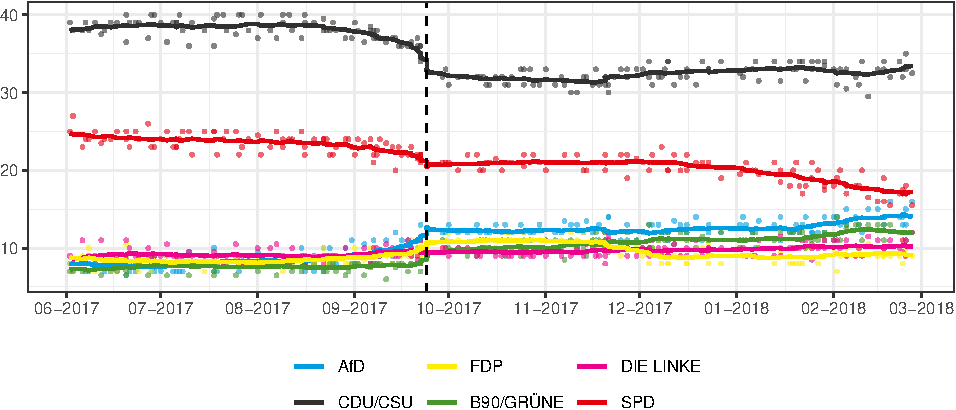
\includegraphics[width=0.8\linewidth]{main_text_files/figure-latex/election polls-1} 

}

\caption{Election polls during the period under review \label{fig:election_polls}}\label{fig:election polls}
\end{figure}

\hypertarget{german-online-news-market}{%
\subsection{German online news market}\label{german-online-news-market}}

\begin{figure}

{\centering \subfloat[Total visits in million (Jan 2018)\label{fig:unnamed-chunk-1-1}]{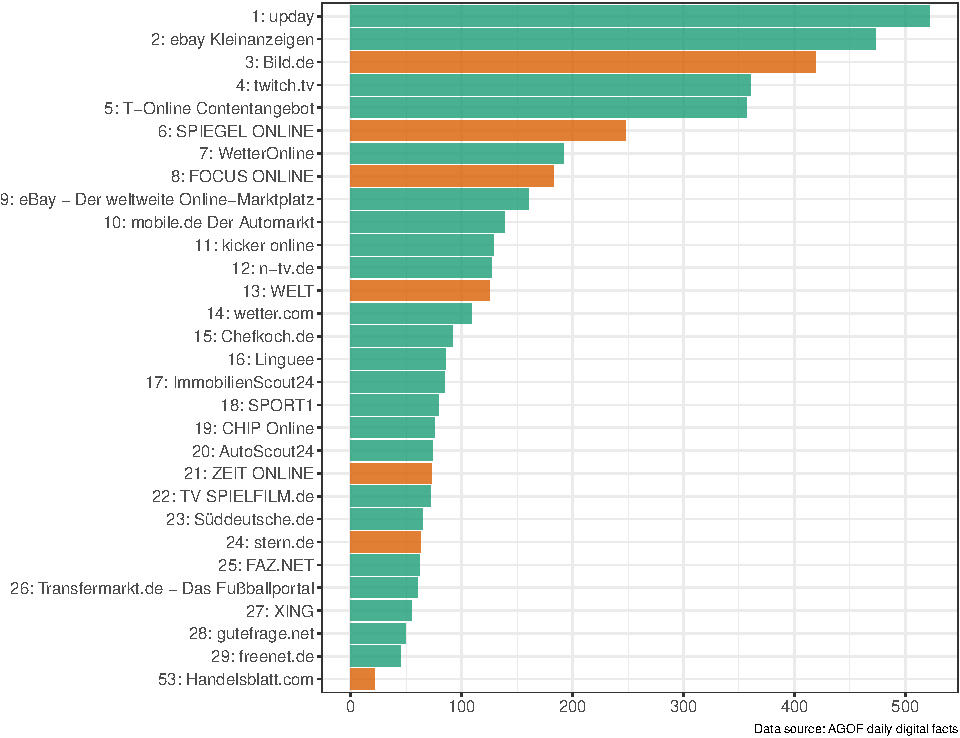
\includegraphics[width=0.49\linewidth]{main_text_files/figure-latex/unnamed-chunk-1-1} }\subfloat[Use of a brand to access news online\label{fig:unnamed-chunk-1-2}]{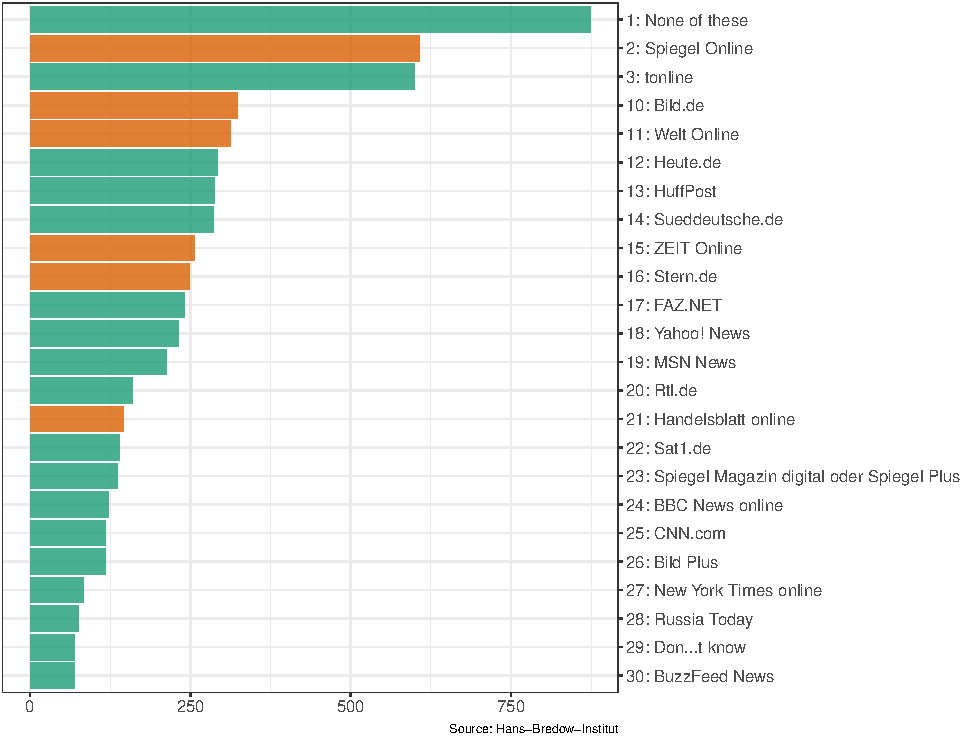
\includegraphics[width=0.49\linewidth]{main_text_files/figure-latex/unnamed-chunk-1-2} }

}

\caption{Selected german news brands \label{fig:news_market}}\label{fig:unnamed-chunk-1}
\end{figure}

The analysis performed in this paper is based on the news articles of
the following news websites: Bild.de, DIE WELT, FOCUS ONLINE,
Handelsblatt, SPIEGEL ONLINE, stern.de, ZEIT ONLINE. As shown in
\autoref{fig:news_market}(a), except for Handelsblatt (position 53),
these media outlets are among the top 30 German online news providers in
the period under review in terms of visits.\footnote{The term visit is
  used to describe the call to a website by a visitor. The visit begins
  as soon as a user generates a page impression (PI) within an offer and
  each additional PI, which the user generates within the offer, belongs
  to this visit.}

The primary source of income for these privately managed media houses is
digital advertising, even though paid content plays an increasingly
important role. However, according to a survey on digital news by the
Reuters Institute (\protect\hyperlink{ref-newman_reuters_2018}{N. Newman
et al. 2018}), only 8\% of respondents pay for online news. The online
survey for German data was undertaken between 19th - 22nd January 2018
by the Hans Bredow Institute\footnote{\url{https://www.hans-bredow-institut.de/de/projekte/reuters-institute-digital-news-survey}}
with a total sample size of 2038 adults (aged 18+) who access news once
a month or more. Among other questions, participants were asked which
news sources they use to access news online.\footnote{The exact question
  was: ``Which of the following brands have you used to access news
  online in the last week (via websites, apps, social media, and other
  forms of Internet access)? Please select all that apply.''} The
results displayed in \autoref{fig:news_market}(b) indicate that the
media used for the analysis play a relevant role in their consumption.

\hypertarget{iii-empirical-analysis}{%
\section{III Empirical analysis}\label{iii-empirical-analysis}}

The empirical strategy used in this paper leverages the structure of the
topic model framework, specifically the Structural Topic Model (STM), to
generate topic distributions for each document which are then used to
measure similarity between documents. The diagram below outlines the
approach in more detail. Section III describes the data sources and how
text data is processed to obtain a multi-dimensional space, where each
dimension corresponds to a word in the document. Subsequently, section
IV uses this so-called document-term matrix as input to calculate each
document's topic distribution using an STM. This, in turn, leads to a
reduction in dimensionality in that each document is now represented as
a distribution over the topics. These document-topic vectors are then
used to calculate the cosine similarity between two documents. The final
Section uses this similarity measure as a dependent variable in a
regression model with different specifications.

\begin{figure}
\centering
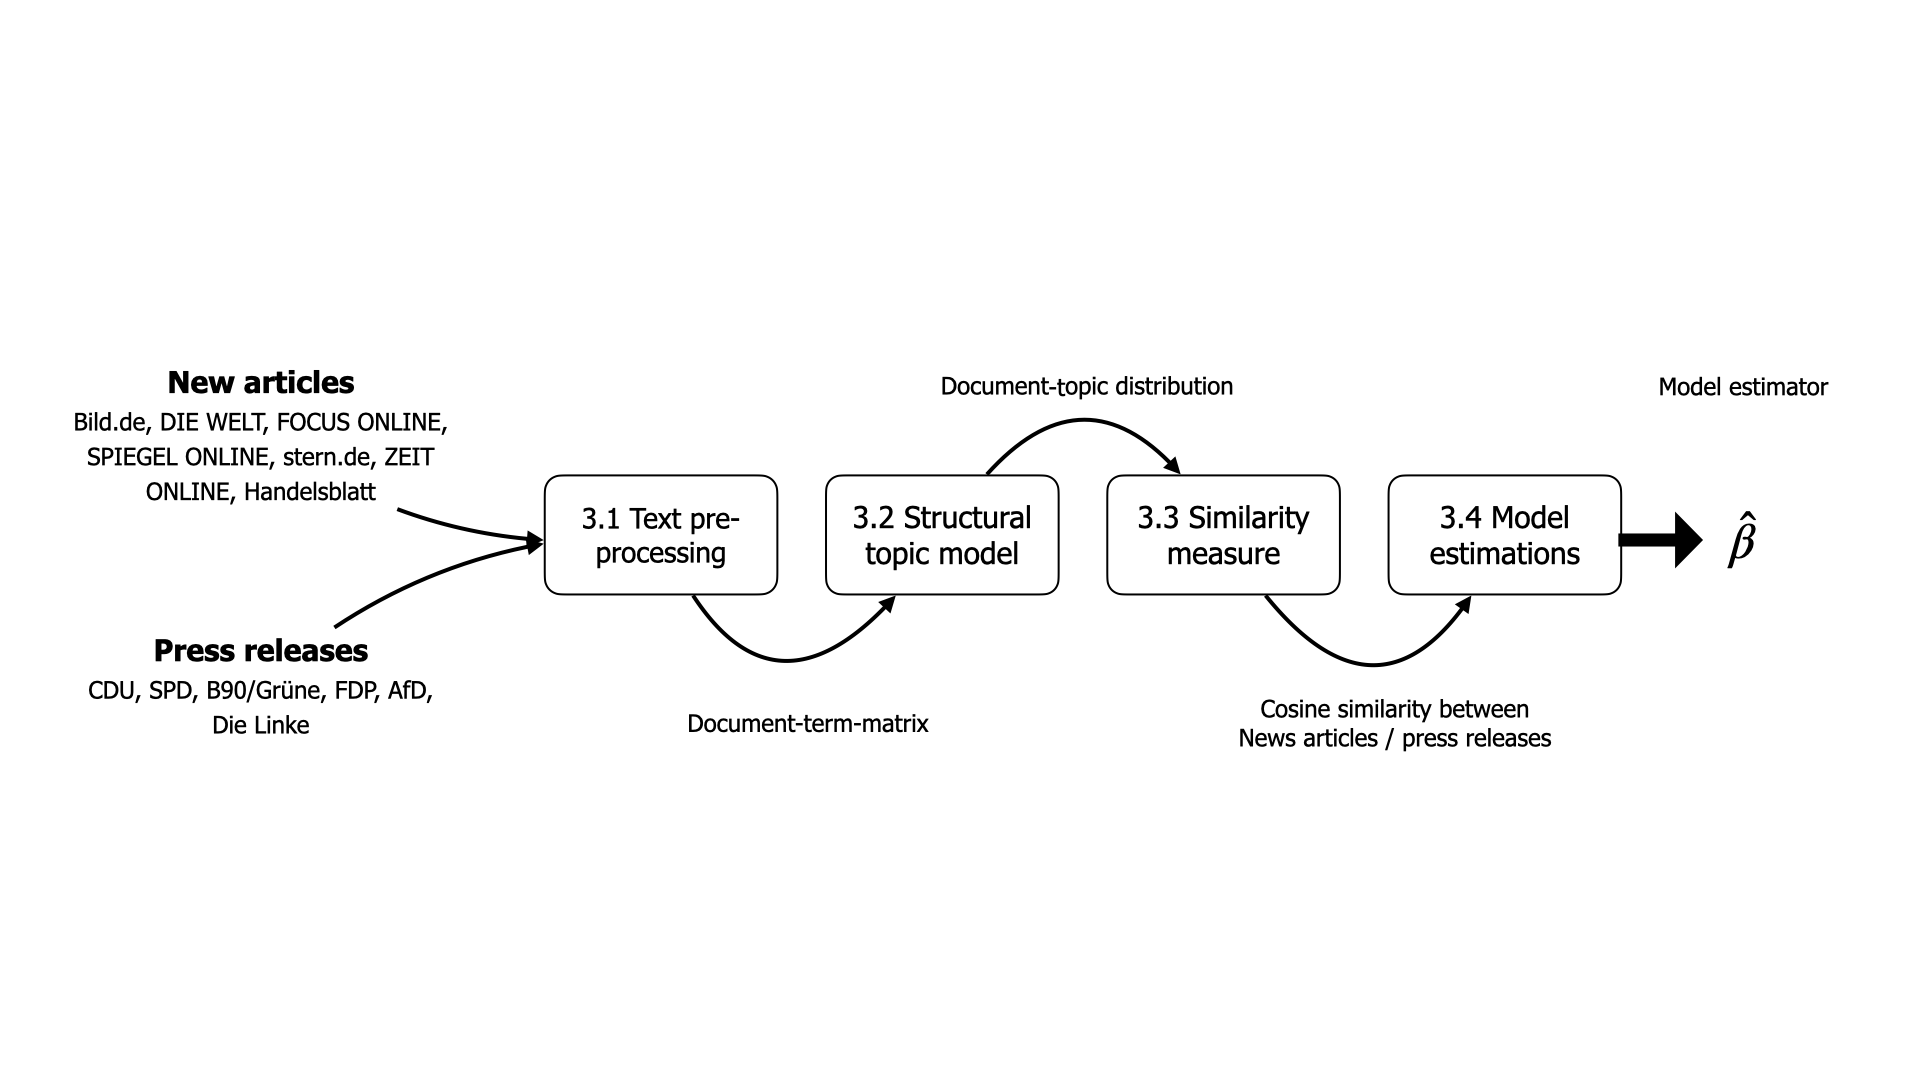
\includegraphics{../figs/high_level_overview.png}
\caption{High level overview}
\end{figure}

\hypertarget{text-data-as-input-for-statistical-modelling}{%
\subsubsection{Text data as input for statistical
modelling}\label{text-data-as-input-for-statistical-modelling}}

I conduct the estimation on a sample of 18,757 online news articles from
the seven German news providers described in the previous
section\footnote{Bild.de, DIE WELT, FOCUS ONLINE, SPIEGEL ONLINE,
  stern.de, ZEIT ONLINE, Handelsblatt} about domestic politics and press
releases of the seven parties that have been in the Bundestag since the
2017 federal elections\footnote{CDU, SPD, B90/Grüne, FDP, AfD, Die Linke}.
Both news articles and press releases are dated from June 1, 2017 to
March 1, 2018.

News articles were scraped from the Webhose.io API.\footnote{For more
  information see
  \url{https://docs.webhose.io/reference\#about-webhose}.} To consider
only news about national politics, the articles were filtered based on
their URL. The press releases were scraped from the public websites of
the political parties and parliamentary groups using an automated
script.\footnote{The scraping code was written in R and can be made
  available on request.}

\autoref{fig:news_distr} shows the distribution of the number of
articles by date and media outlet. There is a high peak around the
federal elections on September 24 and another one shortly after the
failure of the Jamaica coalition talks on November 19 (indicated by the
red dotted lines).\footnote{The peak in July especially for stern.de is
  due to increased reporting about the G20 summit in Hamburg.}
Furthermore, \autoref{fig:news_distr} shows that DIE WELT published the
most articles on domestic policy, followed by stern.de, Handelsblatt and
FOCUS ONLINE.

\begin{figure}

{\centering 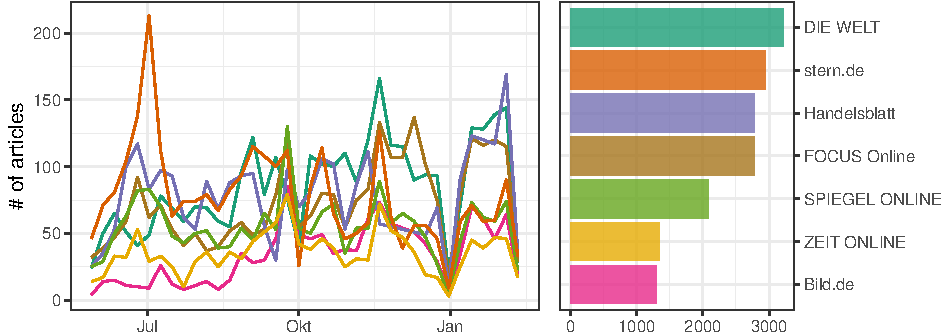
\includegraphics[width=0.8\linewidth]{main_text_files/figure-latex/Distribution of news articles-1} 

}

\caption{Distribution of news articles \label{fig:news_distr}}\label{fig:Distribution of news articles}
\end{figure}

\begin{figure}

{\centering 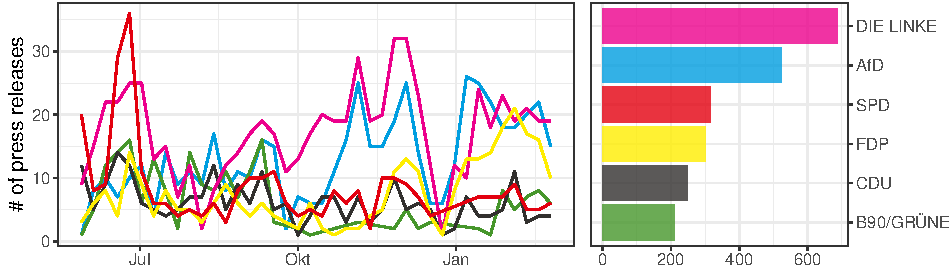
\includegraphics[width=0.8\linewidth]{main_text_files/figure-latex/Distribution of press releases-1} 

}

\caption{Distribution of press releases \label{fig:press_distr}}\label{fig:Distribution of press releases}
\end{figure}

\begin{table}[H]

\caption{\label{tab:table text length}Summary statistics of word counts \label{tab:textlength}}
\centering
\fontsize{7}{9}\selectfont
\begin{tabular}[t]{lrrrrrr}
\toprule
source & n & mean & sd & median & min & max\\
\midrule
\addlinespace[0.3em]
\multicolumn{7}{l}{\textbf{News articles}}\\
\hspace{1em}\cellcolor{gray!6}{Bild.de} & \cellcolor{gray!6}{1303} & \cellcolor{gray!6}{476.07} & \cellcolor{gray!6}{318.28} & \cellcolor{gray!6}{398.0} & \cellcolor{gray!6}{121} & \cellcolor{gray!6}{3710}\\
\hspace{1em}DIE WELT & 3222 & 509.57 & 612.06 & 380.0 & 121 & 14507\\
\hspace{1em}\cellcolor{gray!6}{FOCUS Online} & \cellcolor{gray!6}{2780} & \cellcolor{gray!6}{393.89} & \cellcolor{gray!6}{317.05} & \cellcolor{gray!6}{297.5} & \cellcolor{gray!6}{121} & \cellcolor{gray!6}{5647}\\
\hspace{1em}Handelsblatt & 2785 & 589.51 & 495.82 & 488.0 & 121 & 6899\\
\hspace{1em}\cellcolor{gray!6}{SPIEGEL ONLINE} & \cellcolor{gray!6}{2089} & \cellcolor{gray!6}{539.09} & \cellcolor{gray!6}{415.05} & \cellcolor{gray!6}{413.0} & \cellcolor{gray!6}{121} & \cellcolor{gray!6}{3466}\\
\hspace{1em}stern.de & 2943 & 514.66 & 616.55 & 373.0 & 121 & 9287\\
\hspace{1em}\cellcolor{gray!6}{ZEIT ONLINE} & \cellcolor{gray!6}{1351} & \cellcolor{gray!6}{513.75} & \cellcolor{gray!6}{387.14} & \cellcolor{gray!6}{459.0} & \cellcolor{gray!6}{121} & \cellcolor{gray!6}{8015}\\
\addlinespace[0.3em]
\multicolumn{7}{l}{\textbf{Press releases}}\\
\hspace{1em}AfD & 523 & 212.83 & 72.16 & 196.0 & 103 & 553\\
\hspace{1em}\cellcolor{gray!6}{B90/GRÜNE} & \cellcolor{gray!6}{211} & \cellcolor{gray!6}{229.32} & \cellcolor{gray!6}{63.37} & \cellcolor{gray!6}{219.0} & \cellcolor{gray!6}{104} & \cellcolor{gray!6}{399}\\
\hspace{1em}CDU & 248 & 274.54 & 106.08 & 256.0 & 100 & 1030\\
\hspace{1em}\cellcolor{gray!6}{DIE LINKE} & \cellcolor{gray!6}{686} & \cellcolor{gray!6}{200.47} & \cellcolor{gray!6}{71.78} & \cellcolor{gray!6}{190.0} & \cellcolor{gray!6}{101} & \cellcolor{gray!6}{1048}\\
\hspace{1em}FDP & 301 & 161.90 & 83.78 & 144.0 & 100 & 999\\
\hspace{1em}\cellcolor{gray!6}{SPD} & \cellcolor{gray!6}{315} & \cellcolor{gray!6}{213.41} & \cellcolor{gray!6}{56.16} & \cellcolor{gray!6}{208.0} & \cellcolor{gray!6}{103} & \cellcolor{gray!6}{429}\\
\bottomrule
\end{tabular}
\end{table}

\autoref{tab:textlength} illustrates that, on average, news articles
have a higher word count than the parties' press releases. While for
news articles, the average is between 394 (FOCUS Online) and 590
(Handelsblatt), with press releases, the range is between 162 (FDP) and
275 (CDU). DIE WELT published the article with the most words (14.507) -
the most extended press release has 1.048 words published by DIE LINKE.

Several processing steps have to be performed to make the text
quantifiable to use text as data input for statistical analyses. In
fact, in order to use text as data and reduce the dimensionality to
avoid unnecessary computational complexity and overfitting,
pre-processing the text is a central task in text mining
(\protect\hyperlink{ref-gentzkow_text_2017}{M. Gentzkow, Kelly, and
Taddy} (\protect\hyperlink{ref-gentzkow_text_2017}{2017}),
\protect\hyperlink{ref-bholat_text_2015}{Bholat et al.}
(\protect\hyperlink{ref-bholat_text_2015}{2015})). Intuitively, the term
frequency (tf) of a word measures how important that word may be for
understanding the text. Word clouds are a commonly used visualization
technique in text mining as they translate the tf into the size of the
term in the cloud.

Words like ``die,'' or ``der'' (eng. ``the''), ``and'' (eng. ``and''),
and ``ist'' (eng. ``is'') are extremely common but unrelated to the
quantity of interest. Often called stop words
(\protect\hyperlink{ref-gentzkow_text_2017}{M. Gentzkow, Kelly, and
Taddy 2017}), these terms are essential to the grammatical structure but
typically do not add any additional meaning and can be neglected. The
predefined stop word list from the Snowball project\footnote{\url{http://snowball.tartarus.org/algorithms/german/stop.txt}}
is used together with a customized, domain-specific list of words to
identify and remove these distorting words. Additionally, punctuation
characters (e.g.~., !, ?) and all numbers are removed from the data. The
next step to reduce the dimensionality of text data is to apply an
adequate stemming technique. Stemming is a process by which different
morphological variants of a word are traced back to their common root.
For example, ``voting'' and ``vote'' would be treated as two instances
of the same token after the stemming process. There are many different
techniques for the stemming process. I apply the widely used
Porter-Stemmer algorithm based on a set of shortening rules applied to a
word until it has a minimum number of syllables.\footnote{\url{https://tartarus.org/martin/PorterStemmer/}}

As an example, the following word clouds represent the most frequent
words of the pre-processed articles for Bild.de
(\autoref{fig:wordclouds2}(a)) and press releases of AfD
(\autoref{fig:wordclouds2}(b)). Thus, it becomes evident that these are
texts discussing domestic policy issues. The SPD, in particular, seems
to be highly frequent for Bild.de.

\begin{figure}

{\centering \subfloat[Bild\label{fig:wordclouds2-1}]{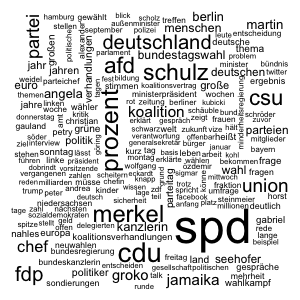
\includegraphics[width=0.4\linewidth]{../figs/wordcloud_bild} }\subfloat[AfD\label{fig:wordclouds2-2}]{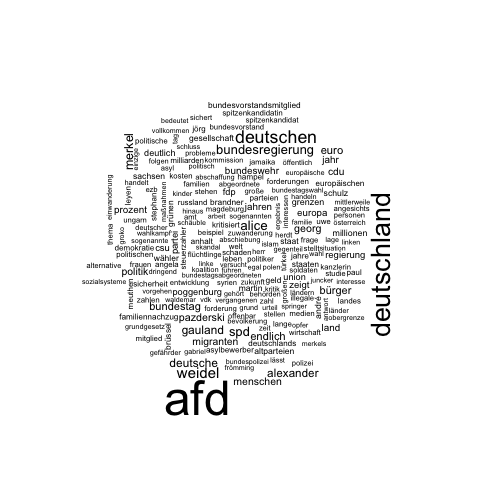
\includegraphics[width=0.4\linewidth]{../figs/wordcloud_afd} }

}

\caption{Wordcloud after pre-processing \label{fig:wordclouds2}}\label{fig:wordclouds2}
\end{figure}

The next step is to divide the entire data set into individual documents
and to represent these documents as a finite list of unique terms. In
this setting, each news article and each press release represents a
document \(d\), whereby each of these documents can be assigned to a
news website or a party. The sum of all documents forms what is called
the corpus. Next, for each document \(d \in \lbrace 1,...,D \rbrace\)
the number of occurrences of term \(v\) in document \(d\) is computed,
in order to obtain the count \(x_{d,v}\), where each unique term in the
corpus is indexed by some \(v \in \lbrace 1,...,V \rbrace\) and where
\(V\) is the number of unique terms. The \(D\) x \(V\) matrix
\(\boldsymbol{X}\) of all such counts is called the document-term
matrix. Each row in this matrix represents a document, and each entry
counts the occurrences of a unique term in that document.
\autoref{table:dtm} provides a sample output of the document-term matrix
used in this paper, where each document is represented by a unique id
(the row name in the example below). This representation is often
referred to as the bag of words model
(\protect\hyperlink{ref-gentzkow_text_2017}{M. Gentzkow, Kelly, and
Taddy 2017}) since it disregards the words' order within a document.

\begin{table}[H]

\caption{\label{tab:Document term matrix}Document-term matrix - sample values \label{table:dtm}}
\centering
\fontsize{7}{9}\selectfont
\begin{tabular}[t]{lrrrrrrr}
\toprule
  & papers & nachzug & sex & stimmten & abgestürzt & gdp & autos\\
\midrule
\cellcolor{gray!6}{14317} & \cellcolor{gray!6}{0} & \cellcolor{gray!6}{0} & \cellcolor{gray!6}{0} & \cellcolor{gray!6}{0} & \cellcolor{gray!6}{0} & \cellcolor{gray!6}{0} & \cellcolor{gray!6}{0}\\
851 & 0 & 0 & 0 & 0 & 0 & 0 & 0\\
\cellcolor{gray!6}{96} & \cellcolor{gray!6}{0} & \cellcolor{gray!6}{0} & \cellcolor{gray!6}{0} & \cellcolor{gray!6}{0} & \cellcolor{gray!6}{0} & \cellcolor{gray!6}{0} & \cellcolor{gray!6}{0}\\
2801 & 0 & 0 & 0 & 0 & 0 & 0 & 0\\
\cellcolor{gray!6}{13257} & \cellcolor{gray!6}{0} & \cellcolor{gray!6}{0} & \cellcolor{gray!6}{0} & \cellcolor{gray!6}{0} & \cellcolor{gray!6}{0} & \cellcolor{gray!6}{0} & \cellcolor{gray!6}{0}\\
\addlinespace
14957 & 0 & 0 & 0 & 0 & 0 & 0 & 0\\
\cellcolor{gray!6}{2308} & \cellcolor{gray!6}{0} & \cellcolor{gray!6}{0} & \cellcolor{gray!6}{0} & \cellcolor{gray!6}{0} & \cellcolor{gray!6}{0} & \cellcolor{gray!6}{0} & \cellcolor{gray!6}{0}\\
3117 & 0 & 0 & 0 & 0 & 0 & 0 & 0\\
\cellcolor{gray!6}{6357} & \cellcolor{gray!6}{0} & \cellcolor{gray!6}{0} & \cellcolor{gray!6}{0} & \cellcolor{gray!6}{1} & \cellcolor{gray!6}{0} & \cellcolor{gray!6}{0} & \cellcolor{gray!6}{0}\\
18293 & 0 & 0 & 0 & 0 & 0 & 0 & 0\\
\bottomrule
\end{tabular}
\end{table}

\hypertarget{a-structural-topic-model-to-identify-the-latent-topics}{%
\subsection{A structural topic model to identify the latent
topics}\label{a-structural-topic-model-to-identify-the-latent-topics}}

Next, a structural topic modeling (STM) developed by
(\protect\hyperlink{ref-roberts_model_2016}{M. E. Roberts, Stewart, and
Airoldi 2016}) is applied to discover the latent topics in the corpus of
press releases and news articles. In general, topic models formalize the
idea that documents are formed by hidden variables (topics) that
generate correlations among observed terms. They belong to the group of
unsupervised generative models, meaning that the true attributes
(topics) cannot be observed. The STM is an extension of the standard
topic modeling technique, labeled as latent Dirichlet allocation (LDA),
which refers to the Bayesian model in Blei, Ng, and Jordan (2003) that
treats each word in a topic and each topic in a document as generated
from a Dirichlet-distributed prior.\footnote{See also
  \protect\hyperlink{ref-griffiths_probabilistic_2002}{Griffiths and
  Steyvers}
  (\protect\hyperlink{ref-griffiths_probabilistic_2002}{2002}),
  \protect\hyperlink{ref-griffiths_finding_2004}{Griffiths and Steyvers}
  (\protect\hyperlink{ref-griffiths_finding_2004}{2004}) and
  \protect\hyperlink{ref-hofmann_probabilistic_1999}{Hofmann}
  (\protect\hyperlink{ref-hofmann_probabilistic_1999}{1999})}

The underlying idea for these models suggests that each topic \(k\)
potentially contains all of the unique terms within the vocabulary \(V\)
with a different probability. Therefore, each topic \(k\) can be
represented as a probability vector \(\phi_k\) over all unique terms
\(V\). Simultaneously, each document \(d\) in the corpus can be
represented as a probability distribution \(\theta_d\) over the \(K\)
topics.

The STM is an extension of the LDA process since it allows covariates of
interest (such as the publication date of a document or its author) to
be included in the prior distributions for both topic proportions
(\(\theta\)) and topic-word distributions (\(\phi\)). This way, STM
offers a method of ``structuring'' the prior distributions in the topic
model, including additional information in the statistical inference
procedure. At the same time, LDA assumes that
\(\theta ~ \text{Dirichlet}(\alpha)\) and
\(\phi ~ \text{Dirichlet}(\beta)\), where \(\alpha\) and \(\beta\) are
fitted with the model.

In order to include the covariates in the statistical inference
procedure, two design matrices of covariates (\(X\) and \(Z\)) are
specified, where each row defines a vector of covariates for a specific
document. \(X\) gives the covariates for topic prevalence resulting in
each document's probability of a topic varies according to \(X\), rather
than resulting from a single common prior. The same applies to \(Z\), in
which the covariates for the word distribution within a topic are
specified. Thus, the underlying data generating process to generate each
word \(w_{d,n}\) in document \(d\) for the \(n^{th}\) word-position can
be described as follows:

\begin{itemize}
\tightlist
\item
  for each document \(i\), draw its distribution of topics \(\theta_d\)
  depending on the metadata included in the model defined in \(X\);
\item
  for each topic \(k\), draw its distribution of words \(\phi_k\)
  depending on the metadata included in the model defined in \(Z\);
\item
  for each word \(n\), draw its topic \(z_n\) based on \(\theta_i\);
\item
  for each word \(n\), draw the term distribution for the selected topic
  \(\phi_{z_{d,n}}\).
\end{itemize}

One crucial assumption for topic models like LDA or STM is the number of
topics (\(K\)) that occur over the entire corpus. Unfortunately, there
is not a ``right'' answer to the number of appropriate topics for a
given corpus (\protect\hyperlink{ref-grimmer_text_2013}{Grimmer and
Stewart 2013}). \protect\hyperlink{ref-roberts_stm:_2016}{M. Roberts,
Stewart, and Tingley} (\protect\hyperlink{ref-roberts_stm:_2016}{2016b})
propose to measure topic quality through a combination of semantic
coherence and exclusivity of words to topics. Semantic coherence is a
criterion developed by
\protect\hyperlink{ref-mimno_optimizing_2011}{Mimno et al.}
(\protect\hyperlink{ref-mimno_optimizing_2011}{2011}). It is closely
related to pointwise mutual information
(\protect\hyperlink{ref-newman_automatic_2010}{D. Newman et al. 2010}):
it is maximized when the most probable words in a given topic are
frequently used in a given topic co-occur together.

The function \(searchK\) from the \(stm\) package
{[}stewart\_bstewartstm\_2021{]} supports the choice of the number of
topics using several automated tests, including the average exclusivity
and semantic coherence and the held-out likelihood
(\protect\hyperlink{ref-wallach_rethinking_2009}{Wallach, Mimno, and
McCallum 2009}) and the residuals
(\protect\hyperlink{ref-taddy_estimation_2012}{Taddy 2012}). This
process revealed that a model with 40 topics best reflects the structure
in the corpus. Furthermore, the author and bi-week dummies of a document
are included as topical prevalence variables. In other words, I assume
that the probability of a topic being included in a news article or a
press release depends on the author and the publication date of that
document. Therefore, I argue that these variables are best suited to
capture temporal and publisher level variation in the documents.

In general, inference of mixed-membership models, such as the one
applied in this paper, has been a thread of research in applied
statistics \protect\hyperlink{ref-braun_variational_2010}{Braun and
McAuliffe} (\protect\hyperlink{ref-braun_variational_2010}{2010}).
However, topic models are usually imprecise as the function to be
optimized has multiple modes so that the model results can be sensitive
to the starting values (e.g., the number of topics and the covariates
influencing the prior distributions). Since an ex-ante valuation is
impossible, I compute various models and compare their posterior
probability to evaluate how results vary for different model
specifications (\protect\hyperlink{ref-roberts_navigating_2016}{M.
Roberts, Stewart, and Tingley 2016a}). I then cross-checked some subset
of assigned topic distributions to evaluate whether the estimates align
with the concept of interest
(\protect\hyperlink{ref-gentzkow_text_2017}{M. Gentzkow, Kelly, and
Taddy 2017}).

\hypertarget{results-of-the-stm}{%
\subsection{Results of the STM}\label{results-of-the-stm}}

As mentioned in the previous section, the generative process of the STM
results in a topic distribution \(\theta_d\) for each document 4d4 over
all topics \(k\) and a word distribution \(\phi_k\) for each topic over
all terms in the vocabulary. Thus, the most probable words of each topic
may help to understand the context of each topic.\footnote{\autoref{table:top_terms}
  gives an overview of the most probable terms for each topic.} However,
since those most probable words are not necessarily the most exclusive
words and only represent a small fraction of the probability
distribution, interpretation should be made cautiously.

For the analysis, the topic distribution of each document is used to
estimate the similarity of documents. \autoref{fig:sample_docs12}
illustrates such a topic distribution of two newspaper articles. The red
numbers display the topic probability (for probabilities\(>= 0.02\)).
News article 1\footnote{Bundeswehr scandal: ex-commander attacks Von Der
  Leyen} shows a definite distribution towards topic 36, for which terms
like Bundeswehr, Soldaten (soldiers), Nato, Verteidigungsministerin
(defense minister) are among the most probable words. News article
2\footnote{Bundestag elections: 42 parties want to be elected to
  parliament.} does not show such a clear tendency towards a single
topic. Topic 40, 18, and 5 are within a close range. However, for all
three topics, similar terms are among the top terms.

Similarly, \autoref{fig:sample_docs34} illustrates the topic
distribution for two press releases randomly chosen from the corpus. For
press release 1\footnote{Lars Herrmann: The danger for Germany and its
  Basic Law is also coming from the left}, topic 24 is the most
probable, containing terms about the G20 Summit, during which left-wing
radicals caused considerable riots. Topic distribution of press article
2\footnote{Trump chooses the path to isolation} shows peaks for topics 6
and 35. The top terms of topic 6 contain the words trump, us, usa,
deutschland (Germany), and präsident (president). Similarly, topic 35
seems to deal with German foreign policy since top terms include words
like eu, deutschland (Germany), europa, and bundesregierung (Federal
Government).

\begin{figure}

{\centering 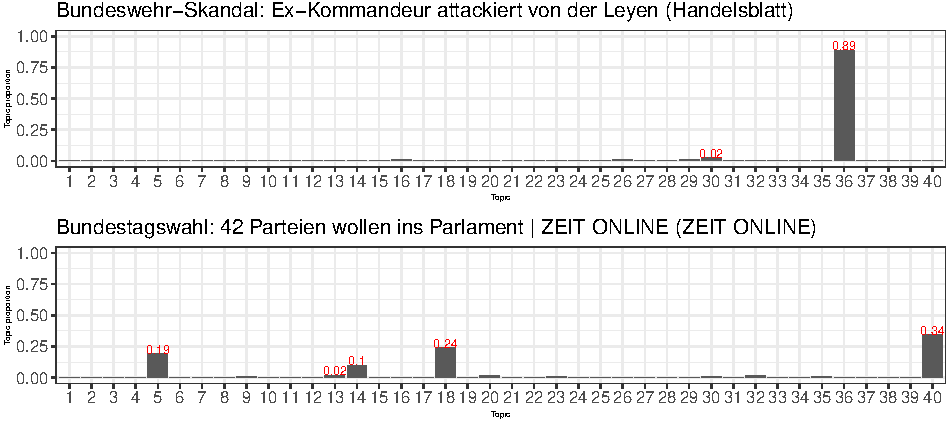
\includegraphics[width=0.9\linewidth]{main_text_files/figure-latex/News articles sample documents-1} 

}

\caption{Topic probability of sample news articles \label{fig:sample_docs12}}\label{fig:News articles sample documents}
\end{figure}

\begin{figure}

{\centering 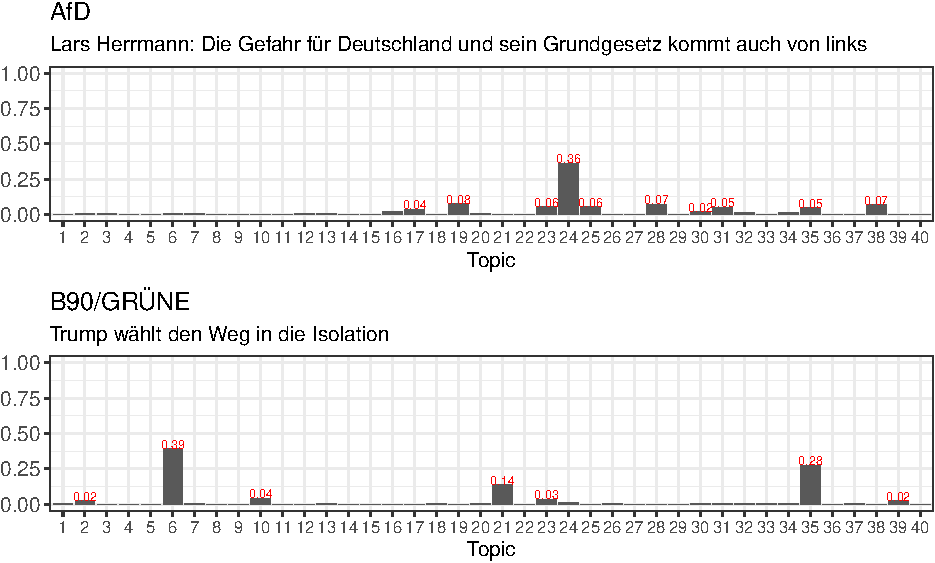
\includegraphics[width=0.9\linewidth]{main_text_files/figure-latex/Press releases sample documents-1} 

}

\caption{Topic probability of sample press releases \label{fig:sample_docs34}}\label{fig:Press releases sample documents}
\end{figure}

Since each document's source and publication date are known, the
probability of specific topics can be analyzed, aggregated by this
metadata. The left chart of \autoref{fig:sample_topics_afd} shows the 15
topics with the highest probability for press releases published by the
AfD. The right side of the figure aggregates the probability by source
and time (in weeks) for two sample topics, displaying how they change
over time in the AfD press releases compared to two sample newspapers.
It becomes clear that topic 9\footnote{translation: afd, party, saxony,
  gauland, parties, pazderski, höcke} is systematically more likely in
the AfD's press releases compared to the two newspapers. There is a
noticeable increase in probability during the election campaign and ends
in a peak on election day itself. For Handelsblatt and Bild.de, too, a
slight increase of probability around election day is discernible.

The top words of topic 38 suggest that it addresses refugees - a topic
for which the AfD has an absolute position. The probability of this
topic increases in the AfD's press releases until about a month before
the election and then levels off somewhat. A similar trend is
discernible in the news articles from Bild.de. The curve from
Handelsblatt is relatively flat and shows no apparent difference between
before and after the election.

\begin{figure}

{\centering 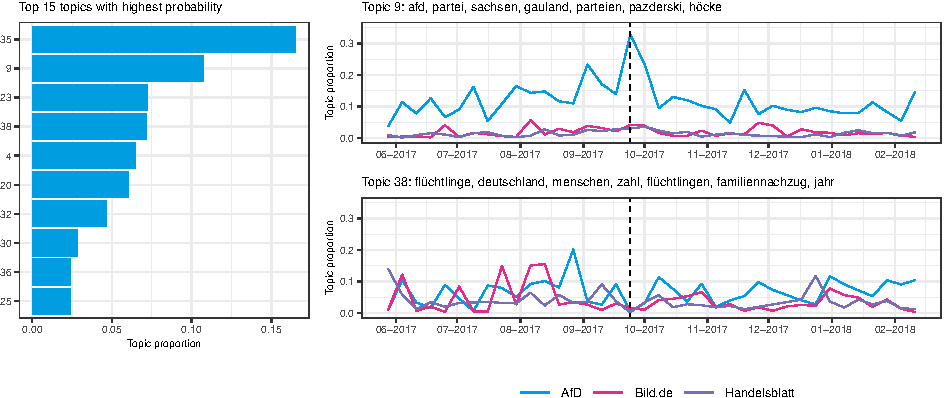
\includegraphics[width=1\linewidth]{main_text_files/figure-latex/Top AfD topics-1} 

}

\caption{Comparison of topic probability - sample topics AfD \label{fig:sample_topics_afd}}\label{fig:Top AfD topics}
\end{figure}

\autoref{fig:sample_topics_fdp} allows a similar analysis for the
aggregated topic distribution in press releases of the FDP. The chart on
the left illustrates that, as in the case of the AfD, topic 35 has the
highest probability in the FDP press releases. Unlike in the case of the
AfD, however, this is followed by topics with more evident temporal
peaks, as shown on the right using two example topics. Topic
10\footnote{translation: diesel, enterprises, germany, cars, german,
  industry, driving bans} has a clear peak for both the newspapers and
the FDP press releases around august 2017. There was a debate about
whether and where driving bans for diesel cars would be introduced.
After the states of Baden-Württemberg and North Rhine-Westphalia
initially filed a lawsuit against this, the court proceedings that would
decide whether driving bans are permissible began in mid-February 2018.
The temporal curve of the FDP shows a further increase in topic
probability at this time, which can also be detected at Handelsblatt. At
Bild.de, however, the topic is only taken up once briefly in August
2017, as only a very low topic probability can be seen after that.

The peak of the probability of topic 39\footnote{translation: fdp,
  grünen, jamaika, cdu, union, grüne, cdu} in all three sources right
after the election reflects the exploratory talks on the possible
formation of a Jamaica coalition, which officially failed on November
19, 2017, after the FDP announced its withdrawal from the negotiations.

\begin{figure}

{\centering 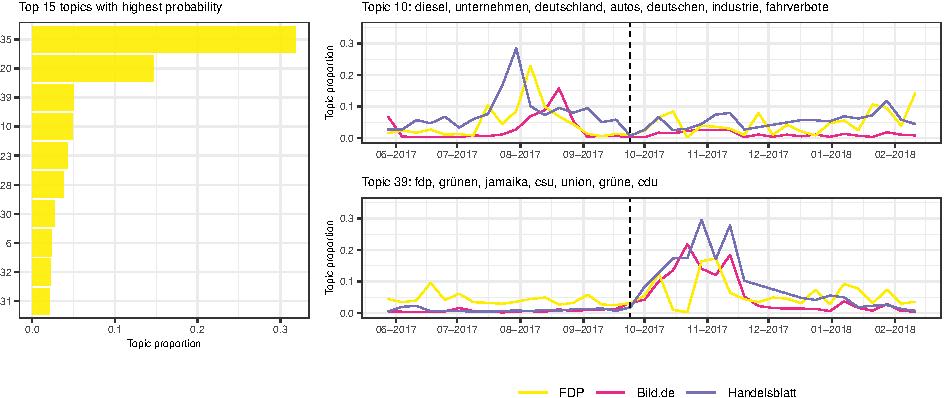
\includegraphics[width=1\linewidth]{main_text_files/figure-latex/Top FDP topics-1} 

}

\caption{Comparison of topic probability - sample topics FDP \label{fig:sample_topics_fdp}}\label{fig:Top FDP topics}
\end{figure}

\hypertarget{similarity-measures}{%
\subsection{Similarity Measures}\label{similarity-measures}}

The topic distributions calculated by the STM are a vectorized
representation of each document as represented by each row in the matrix
in \autoref{table:document_topic_distribution}. Therefore, it is
possible to calculate the similarity between two documents by estimating
the cosine similarity between these vectors.\footnote{For applications
  of cosine similarity to compare of topic model outcomes see e.g.
  \protect\hyperlink{ref-rehs_structural_2020}{Rehs}
  (\protect\hyperlink{ref-rehs_structural_2020}{2020}) and
  \protect\hyperlink{ref-ramage_characterizing_2010}{Ramage, Dumais, and
  Liebling} (\protect\hyperlink{ref-ramage_characterizing_2010}{2010})}

\begin{table}[H]

\caption{\label{tab:Document-topic distribution matrix - sample values}Document-topic distribution matrix \label{table:document_topic_distribution}}
\centering
\fontsize{7}{9}\selectfont
\begin{tabular}[t]{rrrrrrrlr}
\toprule
doc\_index & 1 & 2 & 3 & 4 & 5 & 6 & .. & 40\\
\midrule
\cellcolor{gray!6}{1} & \cellcolor{gray!6}{0.0016} & \cellcolor{gray!6}{0.0453} & \cellcolor{gray!6}{0.0005} & \cellcolor{gray!6}{0.0078} & \cellcolor{gray!6}{0.0151} & \cellcolor{gray!6}{0.0118} & \cellcolor{gray!6}{...} & \cellcolor{gray!6}{0.4376}\\
2 & 0.0041 & 0.0302 & 0.0003 & 0.0044 & 0.0007 & 0.2056 & ... & 0.0006\\
\cellcolor{gray!6}{3} & \cellcolor{gray!6}{0.0043} & \cellcolor{gray!6}{0.0039} & \cellcolor{gray!6}{0.0012} & \cellcolor{gray!6}{0.0003} & \cellcolor{gray!6}{0.0017} & \cellcolor{gray!6}{0.0266} & \cellcolor{gray!6}{...} & \cellcolor{gray!6}{0.0050}\\
4 & 0.0016 & 0.0436 & 0.0006 & 0.0089 & 0.0095 & 0.0126 & ... & 0.5181\\
\cellcolor{gray!6}{5} & \cellcolor{gray!6}{0.0016} & \cellcolor{gray!6}{0.0515} & \cellcolor{gray!6}{0.0002} & \cellcolor{gray!6}{0.0122} & \cellcolor{gray!6}{0.0050} & \cellcolor{gray!6}{0.0121} & \cellcolor{gray!6}{...} & \cellcolor{gray!6}{0.5750}\\
\bottomrule
\end{tabular}
\end{table}

The cosine similarity is the cosine of the angle between two vectors
projected in a multi-dimensional space and is defined between zero and
one; values towards 1 indicate similarity. For example, the cosine
similarity (CS) between document 1 and 2 for \(K=40\) topics can be
calculated as follows.

\[
\text{CS} = \text{cos}(\vec{doc_1},\vec{doc_2})=\frac{\vec{doc_1}*\vec{doc_2}}{||\vec{doc_1}||\vec{doc_2}||}=\frac{\sum^K_{i=1} \vec{doc_{1,i}}\vec{doc_{2,i}}}{\sqrt{\sum^K_{i=1} \vec{doc^2_{1,i}}}, \sqrt{\sum^K_{i=1}\vec{doc^2_{2,i}}}}
\]

For each newspaper, the cosine similarity between all topic-document
distribution pairs between the newspapers articles and the press
releases is calculated if that press release was published within seven
days before the publication date of the news article. Thus, the topic
distribution of news article 1 is compared to press releases 1, 2, 3,
and so on for press releases published within seven days before the news
article. \autoref{table:dataset_structure1} illustrates a sample subset
of the data for DIE WELT.

\begin{table}[H]

\caption{\label{tab:Dataset structure 1}Dataset structure step 1 - DIE WELT \label{table:dataset_structure1}}
\centering
\fontsize{7}{9}\selectfont
\begin{tabular}[t]{llrllll}
\toprule
title1 & title2 & cosine\_sim & source1 & source2 & date1 & date2\\
\midrule
\cellcolor{gray!6}{Bundestagswahl 20...} & \cellcolor{gray!6}{Alexander Gauland...} & \cellcolor{gray!6}{0.33} & \cellcolor{gray!6}{DIE WELT} & \cellcolor{gray!6}{AfD} & \cellcolor{gray!6}{2017-09-25} & \cellcolor{gray!6}{2017-09-19}\\
WELT-Trend: Wird ... & Große Koalition ... & 0.31 & DIE WELT & FDP & 2018-02-07 & 2018-02-05\\
\cellcolor{gray!6}{Befangenheit fest...} & \cellcolor{gray!6}{Der Bundestag bes...} & \cellcolor{gray!6}{0.07} & \cellcolor{gray!6}{DIE WELT} & \cellcolor{gray!6}{SPD} & \cellcolor{gray!6}{2017-06-25} & \cellcolor{gray!6}{2017-06-23}\\
Missbrauch in der... & Eine gerechte Fin... & 0.01 & DIE WELT & DIE LINKE & 2017-07-19 & 2017-07-13\\
\cellcolor{gray!6}{\#CheckdieWahl: „W...} & \cellcolor{gray!6}{Paul Hampel: Dipl...} & \cellcolor{gray!6}{0.23} & \cellcolor{gray!6}{DIE WELT} & \cellcolor{gray!6}{AfD} & \cellcolor{gray!6}{2017-09-22} & \cellcolor{gray!6}{2017-09-22}\\
\bottomrule
\end{tabular}
\end{table}

\autoref{table:cosine_sim_sample_doc}\footnote{Translations: 1) Asylum
  figures 2017 - black-red (synonym for GroKo) introduces upper limit
  through the back door (DIE LINKE) 2) Jörg Meuthen: Not a new GroKo,
  but LoKo - Loser Coalition (AfD) 3) Pension plans of Union and SPD
  worse than expected (FDP) 4) Union and SPD stabilize the extreme
  social injustice in this country (DIE LINKE) 5) Jürgen Pohl: Union and
  SPD agree on policy at the expense of pensioners and East Germans
  (AfD)} displays the most similar documents of the document with the
title \emph{Parteitag, Koalitions-Krimi, Ur-Wahl - Woran kann die GroKo
jetzt noch scheitern? (Bild.de)}.\footnote{Translation: Party
  conference, coalition thriller, primal election - what can fail the
  GroKo now? (Bild.de)}

\begin{table}[H]

\caption{\label{tab:Documents with highest similarity}Most similar documents \label{table:cosine_sim_sample_doc}}
\centering
\fontsize{7}{9}\selectfont
\begin{tabular}[t]{llr}
\toprule
title & source & cos\_sim\\
\midrule
\cellcolor{gray!6}{Asylzahlen 2017 - schwarz-rot führt Obergrenze durch die Hintertür ein} & \cellcolor{gray!6}{DIE LINKE} & \cellcolor{gray!6}{0.542}\\
Jörg Meuthen: Nicht neue GroKo, sondern LoKo – Loser Koalition & AfD & 0.522\\
\cellcolor{gray!6}{Rentenpläne von Union und SPD schlimmer als erwartet} & \cellcolor{gray!6}{FDP} & \cellcolor{gray!6}{0.478}\\
Union und SPD stabilisieren die krasse soziale Ungerechtigkeit in diesem Land & DIE LINKE & 0.401\\
\cellcolor{gray!6}{Jürgen Pohl: Union und SPD verabreden Politik zu Lasten von Rentnern und Ostdeutschen} & \cellcolor{gray!6}{AfD} & \cellcolor{gray!6}{0.388}\\
\bottomrule
\end{tabular}
\end{table}

Next, the mean cosine similarity for each news article publication date
(date1) and party (source2) is estimated to obtain the final data frame
(see \autoref{table:dataset_structure_final}).

\begin{table}[H]

\caption{\label{tab:Dataset structure final}Final dataset structure - DIE WELT \label{table:dataset_structure_final}}
\centering
\fontsize{7}{9}\selectfont
\begin{tabular}[t]{lllr}
\toprule
date1 & source1 & source2 & cos\_sim\\
\midrule
\cellcolor{gray!6}{2017-10-24} & \cellcolor{gray!6}{DIE WELT} & \cellcolor{gray!6}{SPD} & \cellcolor{gray!6}{0.09}\\
2017-06-03 & DIE WELT & DIE LINKE & 0.21\\
\cellcolor{gray!6}{2017-10-09} & \cellcolor{gray!6}{DIE WELT} & \cellcolor{gray!6}{DIE LINKE} & \cellcolor{gray!6}{0.13}\\
2017-11-30 & DIE WELT & SPD & 0.08\\
\cellcolor{gray!6}{2018-01-14} & \cellcolor{gray!6}{DIE WELT} & \cellcolor{gray!6}{CDU} & \cellcolor{gray!6}{0.13}\\
\bottomrule
\end{tabular}
\end{table}

\hypertarget{ols-dummy-regression}{%
\subsection{OLS dummy regression}\label{ols-dummy-regression}}

Finally, cosine similarity can be used as the independent variable in
different model specifications to answer the research questions of this
paper: (a) whether the topics addressed by the parties during the
campaign are echoed in online news, (b) whether there is a difference
for parties, and (c) how and whether topic similarity changes after the
election. First, in \protect\hyperlink{ols-dummy-regression}{OLS dummy
regression}, a OLS model with party dummies is computed for the
pre-election period to examine the extent to which the news outlets pick
up on the parties' issues during election campaigns. Then, in
\protect\hyperlink{regression-discontinuity-model}{Regression
discontinuity model}, a regression discontinuity is specified to test
whether the election day affected overall topic similarity.

To measure whether there is a significant difference in the topic
similarity for each party for a news publisher, a simple OLS regression
is estimated, where the similarity score (\(\ln(\text{CS}_{t})\)) on day
\(t\) between the news articles of that news publisher and the press
releases of a political party \(k\) is the dependent variable and the
political party dummies are the independent variables.

\[
\ln(\text{CS}_{t})=\beta_0+\beta_nD_{t,k-1}+\epsilon_t\text{,}
\]

with \(t\) = date\footnote{date1 in
  \autoref{table:dataset_structure_final}}, \(k\) = political
party\footnote{source2 in \autoref{table:dataset_structure_final}}

\hypertarget{ols-dummy-results}{%
\subsubsection{OLS dummy results}\label{ols-dummy-results}}

The columns in \autoref{table:results_ols} report the results for each
new publisher.\footnote{All regression output tables are created using
  \protect\hyperlink{ref-hlavac_stargazer_2018}{Hlavac}
  (\protect\hyperlink{ref-hlavac_stargazer_2018}{2018})} Since the
dependent variable is log-transformed, the \(\%\) impact of \(D\) on
\(Y\) can be estimated using \(exp(\hat\beta)-1\). E.g., since the
transformed coefficient for \(D_{B90/GRÜNE}\) in the first column -
representing the model for DIE WELT - is \(-0.279\), a switch from 0 to
1 can be interpreted as a \(36.4\%\) decrease of topic similarity for
B90/GRÜNE compared to AfD (the base dummy group), holding everything
else equal. In other words: Compared to AfD, the similarity of topics of
DIE WELT and B90/GRÜNE is \(36.4\%\) lower.
\autoref{fig:coeff_ols_dummy} plots the transformed coefficients for all
newspaper/party pairs (insignificant coefficients are shown with low
opacity). In general, for all newspapers - except for Handelsblatt - the
topic similarity is significantly less between the news articles of that
newspaper and press releases of political parties compared to press
releases of the AfD. The most evident difference for all parties exists
for Bild.de, followed by FOCUS ONLINE and DIE WELT. In the case of
Handelsblatt no significant difference can be found for CDU/CSU,
B90/GRÜNE and SPD (compared to AfD). However, the positive coefficients
of DIE LINKE indicate that the topics discussed in press releases of
that party and the articles of Handelsblatt are significantly similar
compared to the press releases of the AfD.

\begin{figure}

{\centering 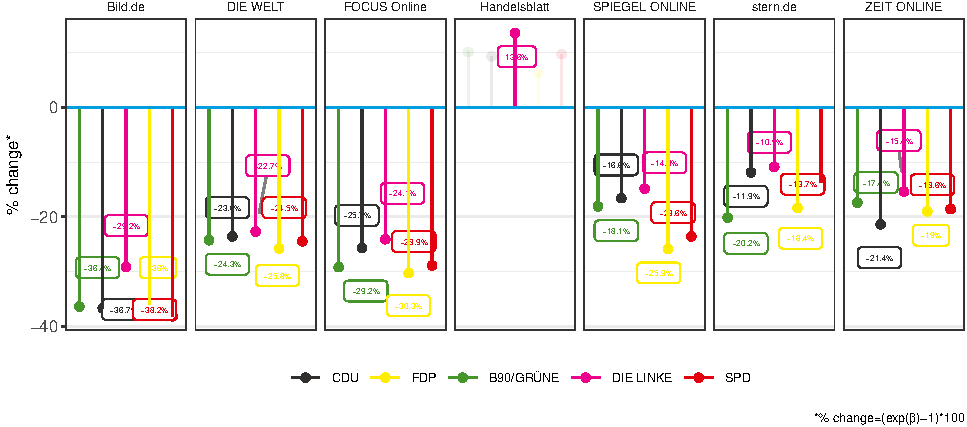
\includegraphics[width=1\linewidth]{main_text_files/figure-latex/Plot coefficients - simple dummy-1} 

}

\caption{Coefficients of OLS dummy regression \label{fig:coeff_ols_dummy}}\label{fig:Plot coefficients - simple dummy}
\end{figure}

\begin{table}[!htbp] \centering    \caption{Results from the OLS dummy regression}    \label{table:results_ols}  \resizebox{0.99\textwidth}{!}{\begin{tabular}{@{\extracolsep{5pt}}lccccccc}  \\[-1.8ex]\hline  \hline \\[-1.8ex]   & \multicolumn{7}{c}{\textit{Dependent variable:}} \\  \cline{2-8}  \\[-1.8ex] & \multicolumn{7}{c}{Cosine similarity of topic distribution} \\   & DIE WELT & stern.de & ZEIT ONLINE & Handelsblatt & FOCUS Online & Bild.de & SPIEGEL ONLINE \\  \\[-1.8ex] & (1) & (2) & (3) & (4) & (5) & (6) & (7)\\  \hline \\[-1.8ex]   B90/GRÜNE & $-$0.279$^{***}$ & $-$0.226$^{***}$ & $-$0.192$^{***}$ & 0.096 & $-$0.345$^{***}$ & $-$0.452$^{***}$ & $-$0.199$^{***}$ \\    & (0.050) & (0.054) & (0.065) & (0.061) & (0.058) & (0.093) & (0.067) \\    & & & & & & & \\   CDU & $-$0.270$^{***}$ & $-$0.127$^{**}$ & $-$0.241$^{***}$ & 0.089 & $-$0.297$^{***}$ & $-$0.457$^{***}$ & $-$0.181$^{***}$ \\    & (0.050) & (0.053) & (0.065) & (0.060) & (0.058) & (0.093) & (0.067) \\    & & & & & & & \\   DIE LINKE & $-$0.257$^{***}$ & $-$0.116$^{**}$ & $-$0.167$^{**}$ & 0.127$^{**}$ & $-$0.275$^{***}$ & $-$0.345$^{***}$ & $-$0.162$^{**}$ \\    & (0.050) & (0.053) & (0.065) & (0.060) & (0.058) & (0.093) & (0.067) \\    & & & & & & & \\   FDP & $-$0.299$^{***}$ & $-$0.204$^{***}$ & $-$0.210$^{***}$ & 0.061 & $-$0.361$^{***}$ & $-$0.446$^{***}$ & $-$0.299$^{***}$ \\    & (0.050) & (0.053) & (0.065) & (0.060) & (0.058) & (0.093) & (0.067) \\    & & & & & & & \\   SPD & $-$0.282$^{***}$ & $-$0.147$^{***}$ & $-$0.206$^{***}$ & 0.093 & $-$0.341$^{***}$ & $-$0.481$^{***}$ & $-$0.270$^{***}$ \\    & (0.050) & (0.053) & (0.065) & (0.060) & (0.058) & (0.093) & (0.067) \\    & & & & & & & \\   Constant & $-$1.705$^{***}$ & $-$2.021$^{***}$ & $-$1.641$^{***}$ & $-$1.876$^{***}$ & $-$1.793$^{***}$ & $-$1.680$^{***}$ & $-$1.880$^{***}$ \\    & (0.036) & (0.038) & (0.046) & (0.043) & (0.041) & (0.066) & (0.048) \\    & & & & & & & \\  \hline \\[-1.8ex]  Observations & 683 & 689 & 671 & 641 & 695 & 594 & 695 \\  R$^{2}$ & 0.071 & 0.031 & 0.026 & 0.008 & 0.074 & 0.062 & 0.034 \\  Adjusted R$^{2}$ & 0.064 & 0.024 & 0.019 & 0.0003 & 0.068 & 0.054 & 0.027 \\  Residual Std. Error & 0.379 (df = 677) & 0.406 (df = 683) & 0.485 (df = 665) & 0.442 (df = 635) & 0.440 (df = 689) & 0.655 (df = 588) & 0.512 (df = 689) \\  F Statistic & 10.295$^{***}$ (df = 5; 677) & 4.436$^{***}$ (df = 5; 683) & 3.554$^{***}$ (df = 5; 665) & 1.038 (df = 5; 635) & 11.089$^{***}$ (df = 5; 689) & 7.824$^{***}$ (df = 5; 588) & 4.890$^{***}$ (df = 5; 689) \\  \hline  \hline \\[-1.8ex]  \textit{Note:}  & \multicolumn{7}{r}{$^{*}$p$<$0.1; $^{**}$p$<$0.05; $^{***}$p$<$0.01} \\  \end{tabular}}  \end{table}

\hypertarget{regression-discontinuity-model}{%
\subsection{Regression discontinuity
model}\label{regression-discontinuity-model}}

I assume that news publishers report differently during election
campaigns and that the election day introduces a change in the
reporting. The underlying dynamic of this assumption coincides with the
basic idea of regression discontinuity design (RDD). Therefore, an RDD
is applied to identify the short-term effect of the election on the
topic similarity between newspaper articles and press releases. The RDD
was designed by
\protect\hyperlink{ref-thistlethwaite_regression-discontinuity_1960}{Thistlethwaite
and Campbell}
(\protect\hyperlink{ref-thistlethwaite_regression-discontinuity_1960}{1960})
and formalized by \protect\hyperlink{ref-hahn_identification_2001}{Hahn,
Todd, and Van der Klaauw}
(\protect\hyperlink{ref-hahn_identification_2001}{2001}) to measure the
effect of a treatment in a non-experimental setting, where the treatment
is defined as a discontinuous function of a continuous, observed
variable (the `running' or `forcing' variable). Like
\protect\hyperlink{ref-thistlethwaite_regression-discontinuity_1960}{Thistlethwaite
and Campbell}
(\protect\hyperlink{ref-thistlethwaite_regression-discontinuity_1960}{1960}),
who estimated the effect of receiving the National Merit Scholarship on
future academic outcomes, early studies that rely on RD designs estimate
the effects of certain thresholds of a running variable on educational
outcomes (i.e., financial aid
(\protect\hyperlink{ref-van_der_klaauw_estimating_2002}{Klaauw 2002}) or
class size (\protect\hyperlink{ref-angrist_using_1999}{Angrist and Lavy
1999})). Following these early studies in education, the RDD has
received attention in a broader range of the economic literature,
including labor economics, political economy, health economics, and
environmental economics. Compared to alternative quasi-experimental
estimators like difference-in-difference and matching techniques, RDD is
the estimator with the most significant internal validity
(\protect\hyperlink{ref-lee_regression_2010}{Lee and Lemieux 2010}).

While RDD was applied initially in cross-sectional studies, an
increasing number of studies, especially in environmental and energy
economics, have adapted the framework to time series applications. In
these studies, time is the running variable, and treatment begins at a
particular threshold in time. A significant conceptual difference
between regression discontinuity (RD) and regression discontinuity in
time (RDiT) lies in the possible interpretation of the results. Since in
RDiT, the running variable of time is not random eliminates the
interpretation of local randomization. As noted by
\protect\hyperlink{ref-jacob_practical_2012}{Jacob et al.}
(\protect\hyperlink{ref-jacob_practical_2012}{2012}), although some
researchers have focused on this interpretation of local randomization,
in which the treatment status within a small neighborhood around the
threshold can essentially be compared to a roll of the dice
(\protect\hyperlink{ref-lee_regression_2010}{Lee and Lemieux 2010}),
others have emphasized that RD is characterized by discontinuity at a
threshold (\protect\hyperlink{ref-hahn_identification_2001}{Hahn, Todd,
and Van der Klaauw 2001}). Thus, to the extent that the RD framework is
simply another quasi-experimental framework (one that uses
discontinuity), RDiT is conceptually similar to RD.

In this paper, the date is the running variable, the election day is the
treatment, and news publishers are the units that receive the treatment.
A sharp regression design is used since the running variable (date)
ultimately determines the treatment (election day). Thus, a news
publisher's probability of receiving a treatment jumps from 0 to 1 at
the cutoff. Specifically, the following equation is estimated:

\[
\ln(\text{CS}_{t})=\beta_0+\beta_1T_t+f(W_t)+\epsilon_t
\] where

\[
T_t = 
\begin{cases}
1, & \text{ if date } \geq \text{election date} \\
0, & \text{ if date } < \text{election date}
\end{cases}
\]

The running variable \(W_t\) is the time difference between date \(i\)
and the election date (in days), such that \(\beta_1\) is the average
treatment effect for observations with \(W_t = 0\) (the election date).
In other words, \(\beta_1\) gives the average change of the similarity
between news publisher content and press releases after the election
day. Identification in the RD model comes from assuming that the
underlying, potentially endogenous relationship between \(\epsilon_t\)
and the date is eliminated by the flexible function \(f(.)\). In
particular, the relationship between \(\epsilon_t\) and the date must
not change discontinuously on or near the election date.

Following \protect\hyperlink{ref-imbens_regression_2008}{Imbens and
Lemieux} (\protect\hyperlink{ref-imbens_regression_2008}{2008}) I
estimate a local linear regression model of the form:

\[
\ln(\text{CS}_{t})=\beta_0+\beta_1T_t+\beta_2W_t+\beta_3W_t*T_t+\epsilon_t
\]

In this specification (results are shown in
\protect\hyperlink{RDiT-Results}{RDiT Results}), the function \(f(W_t)\)
is specified as \(\beta_2W_t+\beta_3W_t*T_t\), where by \(W_t*T_t\) is
assumed that in addition to the intercept (captured by the treatment
effect \(T_t\)), the slope also changes after the election day. The
interaction term, together with \(W_t\), should absorb any smooth
relationship between the date and \(\epsilon_t\) in the days surrounding
the election day. Thus, if the RD assumption is valid (i.e.,
\(\epsilon_t\) does not change discontinuously at the election day), the
estimate of \(\beta_1\), the coefficient of interest, will be unbiased
even without further controls.

However, in section \protect\hyperlink{RDiT-dummy-results}{RDiT dummy
results} dummy variables for each party \(k\) (\(D_{t,k-1}\)) are
included, to test the assumption that the effect of the election day on
topic similarity differs for different parties. Here again, the
interaction term \(T_t*D_{t,k-1}\) allows for a slope change depending
on the party. Thus \(\beta_5\) gives the average treatment effect for
each newspaper/party pair.

\[
\ln(\text{CS}_{t})=\beta_0+\beta_1T_t+\beta_2W_{t}+\beta_3W_t*T_t+\beta_4D_{t,k-1}+\beta_5T_t*D_{t,k-1}+\epsilon_t
\]

I specify a uniform kernel
(\protect\hyperlink{ref-lee_regression_2010}{Lee and Lemieux 2010}) and
use a bandwidth of 115 days on each side of the election day threshold.
The election took place on September 24, 2017, so the sample includes
dates between June 1, 2017, and January 17, 2018. Since the
identification strategy only attempts to estimate \(\beta\) at \(W_t=0\)
(the election day), no additional dates beyond the 115-day bandwidth
enter the sample. Alternative specifications with varying bandwidths led
to similar results.

\hypertarget{rdit-results}{%
\subsubsection{RDiT Results}\label{rdit-results}}

\autoref{table:results_rd1} shows the results of this estimation. The
negative and significant values for \(\beta_1\) indicate that - holding
the time constant - the election day is associated with a decrease in
topic similarity for DIE WELT, stern.de, ZEIT ONLINE, and Handelsblatt.
Since I am interested in the treatment effect at the cutoff point
(remember that \(W_t=0\) for the election day) and since

\[
\frac{\Delta Y}{\Delta T}=\beta_1+\beta_3W,
\]

\(\beta_1\) can be interpreted as the change in topic similarity with
respect to the election day. Similarly to the interpretation in
\protect\hyperlink{OLS-dummy-results}{OLS dummy results}, the the \%
impact of \(T\) on \(Y\) can be estimated as \(exp(\beta_1)-1\).
\autoref{fig:coeff_rdit} shows the transformed coefficients for all
newspapers: The negative effect of the election day on the topic
similarity is strongest for Handelsblatt (\textasciitilde21.5\%
decrease), followed by DIE WELT (\textasciitilde15.6\% decrease), ZEIT
ONLINE (\textasciitilde13.5\% decrease) and stern.de
(\textasciitilde11.1\% decrease).

\begin{table}[!htbp] \centering    \caption{Results from the RDiT model}    \label{table:results_rd1}  \resizebox{0.99\textwidth}{!}{\begin{tabular}{@{\extracolsep{5pt}}lccccccc}  \\[-1.8ex]\hline  \hline \\[-1.8ex]   & \multicolumn{7}{c}{\textit{Dependent variable:}} \\  \cline{2-8}  \\[-1.8ex] & \multicolumn{7}{c}{Cosine similarity of topic distribution} \\   & DIE WELT & stern.de & ZEIT ONLINE & Handelsblatt & FOCUS Online & Bild.de & SPIEGEL ONLINE \\  \\[-1.8ex] & (1) & (2) & (3) & (4) & (5) & (6) & (7)\\  \hline \\[-1.8ex]   T & $-$0.169$^{***}$ & $-$0.118$^{**}$ & $-$0.145$^{**}$ & $-$0.242$^{***}$ & $-$0.058 & $-$0.032 & 0.035 \\    & (0.045) & (0.057) & (0.065) & (0.060) & (0.048) & (0.066) & (0.055) \\    & & & & & & & \\   W & $-$0.001$^{*}$ & $-$0.0005 & $-$0.002$^{***}$ & $-$0.0003 & $-$0.001 & $-$0.001 & $-$0.002$^{***}$ \\    & (0.0004) & (0.001) & (0.001) & (0.001) & (0.0005) & (0.001) & (0.001) \\    & & & & & & & \\   TTRUE:W & 0.003$^{***}$ & 0.003$^{***}$ & 0.002$^{*}$ & 0.005$^{***}$ & 0.002$^{**}$ & 0.003$^{***}$ & 0.003$^{***}$ \\    & (0.001) & (0.001) & (0.001) & (0.001) & (0.001) & (0.001) & (0.001) \\    & & & & & & & \\   Constant & $-$1.972$^{***}$ & $-$2.181$^{***}$ & $-$1.927$^{***}$ & $-$1.812$^{***}$ & $-$2.091$^{***}$ & $-$2.080$^{***}$ & $-$2.160$^{***}$ \\    & (0.029) & (0.036) & (0.045) & (0.043) & (0.033) & (0.046) & (0.038) \\    & & & & & & & \\  \hline \\[-1.8ex]  Observations & 1,212 & 1,218 & 1,244 & 1,046 & 1,268 & 1,161 & 1,264 \\  R$^{2}$ & 0.031 & 0.011 & 0.059 & 0.035 & 0.005 & 0.013 & 0.009 \\  Adjusted R$^{2}$ & 0.028 & 0.009 & 0.056 & 0.032 & 0.003 & 0.011 & 0.007 \\  Residual Std. Error & 0.377 (df = 1208) & 0.471 (df = 1214) & 0.586 (df = 1240) & 0.491 (df = 1042) & 0.427 (df = 1264) & 0.579 (df = 1157) & 0.495 (df = 1260) \\  F Statistic & 12.805$^{***}$ (df = 3; 1208) & 4.655$^{***}$ (df = 3; 1214) & 25.810$^{***}$ (df = 3; 1240) & 12.532$^{***}$ (df = 3; 1042) & 2.134$^{*}$ (df = 3; 1264) & 5.154$^{***}$ (df = 3; 1157) & 3.820$^{***}$ (df = 3; 1260) \\  \hline  \hline \\[-1.8ex]  \textit{Note:}  & \multicolumn{7}{r}{$^{*}$p$<$0.1; $^{**}$p$<$0.05; $^{***}$p$<$0.01} \\  \end{tabular}}  \end{table}

\begin{figure}

{\centering 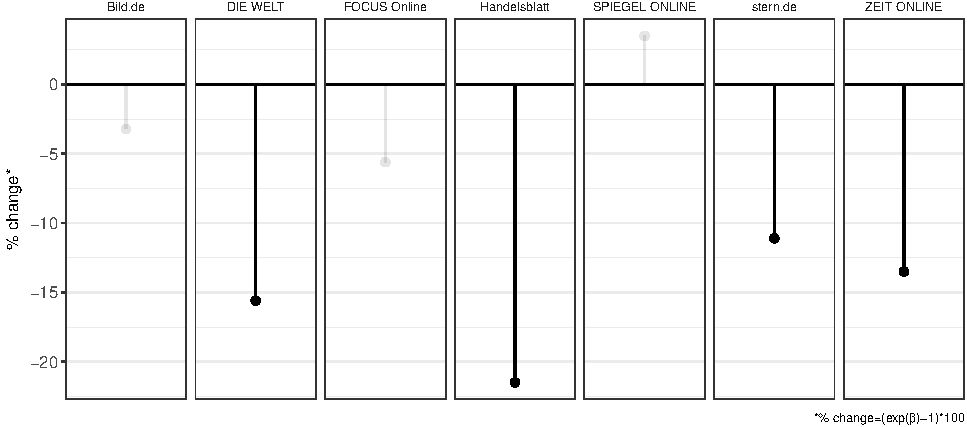
\includegraphics[width=1\linewidth]{main_text_files/figure-latex/Plot coefficients - RDiT-1} 

}

\caption{Treatment effect of RDiT regression \label{fig:coeff_rdit}}\label{fig:Plot coefficients - RDiT}
\end{figure}

\hypertarget{rdit-dummy-results}{%
\subsubsection{RDiT dummy results}\label{rdit-dummy-results}}

As mentioned above, I assume that the effect of the election day on the
topic similarity is different for different parties.
\autoref{fig:mean_cosine_sim_rd_example} visually captures the treatment
effect for two sample news publishers Handelsblatt and Bild.de. It
reveals a treatment effect around the cutoff point for Handelsblatt and
CDU, FDP, and B90/GRÜNE: For all pairs, the topic similarity decreases
right after the election day. The same is true for Bild.de and AfD (see
\autoref{fig:mean_cosine_sim_rd} for all news publishers). Thus, a
positive effect can only be found for Bild.de and B90/GRÜNE and Bild.de
and CDU. The figure also illustrates a slope change after the election
day for nearly all newspaper/party pairs.

\begin{figure}

{\centering 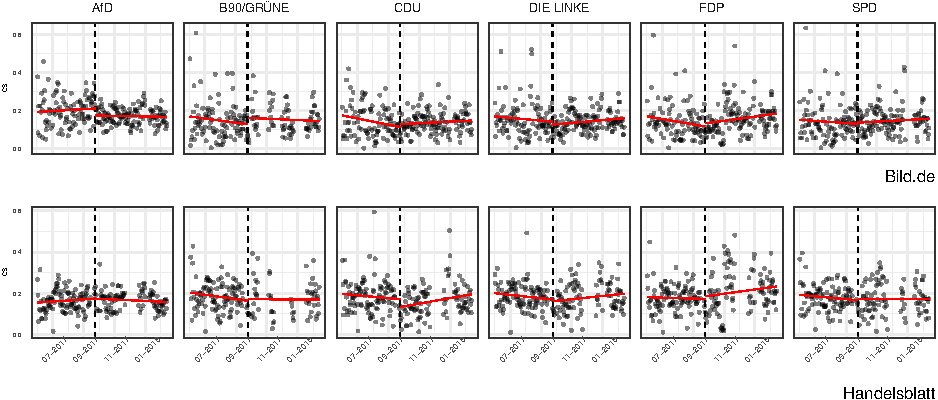
\includegraphics[width=1\linewidth]{main_text_files/figure-latex/Daily mean cosine similarity - rd example-1} 

}

\caption{Log of mean cosine similarity between newspaper/press articles pairs - with cutoff value \label{fig:mean_cosine_sim_rd_example}}\label{fig:Daily mean cosine similarity - rd example}
\end{figure}

\autoref{table:results_rd2} outputs the results for all newspaper
models. The coefficients for the treatment variables (e.g.,
``TTRUE:B90/GRÜNE'') show the effect of the election day's effect on the
topic similarity depending on the party for a given \(W\). This effect
can be illustrated using Handelsblatt and B90/GRÜNE as an example and
comparing the model equation for \(D_{B90/GRÜNE} = 1\) and
\(D_{B90/GRÜNE} = 0\) for \(W=0\). For \(D_{B90/GRÜNE} = 1\) the
equation is

\[
\ln(\text{CS})=-1.896+(-0.091)T+(-0.260)T,
\]

whereas for \(D_{B90/GRÜNE} = 0\) it is

\[
\ln(\text{CS})=-1.896+(-0.091)T.
\]

In other words, when \(D_{B90/GRÜNE}\) switches from 0 to 1, the
treatment effect decreases by \(0.260\) compared to the base dummy group
AfD, for which the treatment effect is \(-0.091\). Again, since I
estimate a log-linear regression model, the coefficient should be
transformed using \(\exp(-0.260)-1 = -0.229\). Therefore, the topic
similarity between Handelsblatt and B90/GRÜNE decreases right after the
election day by \(22.9\%\) compared to AfD (the base dummy group).

\begin{table}[!htbp] \centering    \caption{Results from the regression discontinuity model}    \label{table:results_rd2}  \resizebox{0.99\textwidth}{!}{\begin{tabular}{@{\extracolsep{5pt}}lccccccc}  \\[-1.8ex]\hline  \hline \\[-1.8ex]   & \multicolumn{7}{c}{\textit{Dependent variable:}} \\  \cline{2-8}  \\[-1.8ex] & \multicolumn{7}{c}{Cosine similarity of topic distribution} \\   & DIE WELT & stern.de & ZEIT ONLINE & Handelsblatt & FOCUS Online & Bild.de & SPIEGEL ONLINE \\  \\[-1.8ex] & (1) & (2) & (3) & (4) & (5) & (6) & (7)\\  \hline \\[-1.8ex]   T & $-$0.167$^{***}$ & $-$0.048 & $-$0.038 & $-$0.091 & $-$0.072 & $-$0.187$^{*}$ & 0.076 \\    & (0.063) & (0.081) & (0.096) & (0.090) & (0.068) & (0.097) & (0.081) \\    & & & & & & & \\   W & $-$0.001$^{*}$ & $-$0.0005 & $-$0.002$^{***}$ & $-$0.0003 & $-$0.001 & $-$0.001 & $-$0.002$^{***}$ \\    & (0.0004) & (0.001) & (0.001) & (0.001) & (0.0005) & (0.001) & (0.001) \\    & & & & & & & \\   B90/GRÜNE & $-$0.267$^{***}$ & $-$0.215$^{***}$ & $-$0.180$^{**}$ & 0.105 & $-$0.337$^{***}$ & $-$0.445$^{***}$ & $-$0.186$^{***}$ \\    & (0.048) & (0.062) & (0.078) & (0.067) & (0.054) & (0.081) & (0.064) \\    & & & & & & & \\   CDU & $-$0.259$^{***}$ & $-$0.115$^{*}$ & $-$0.232$^{***}$ & 0.098 & $-$0.288$^{***}$ & $-$0.450$^{***}$ & $-$0.170$^{***}$ \\    & (0.048) & (0.061) & (0.078) & (0.067) & (0.054) & (0.081) & (0.064) \\    & & & & & & & \\   DIE LINKE & $-$0.251$^{***}$ & $-$0.109$^{*}$ & $-$0.160$^{**}$ & 0.134$^{**}$ & $-$0.270$^{***}$ & $-$0.342$^{***}$ & $-$0.156$^{**}$ \\    & (0.048) & (0.061) & (0.078) & (0.067) & (0.054) & (0.081) & (0.064) \\    & & & & & & & \\   FDP & $-$0.291$^{***}$ & $-$0.195$^{***}$ & $-$0.201$^{***}$ & 0.069 & $-$0.355$^{***}$ & $-$0.441$^{***}$ & $-$0.292$^{***}$ \\    & (0.048) & (0.061) & (0.078) & (0.067) & (0.054) & (0.081) & (0.064) \\    & & & & & & & \\   SPD & $-$0.278$^{***}$ & $-$0.143$^{**}$ & $-$0.201$^{***}$ & 0.098 & $-$0.339$^{***}$ & $-$0.479$^{***}$ & $-$0.266$^{***}$ \\    & (0.048) & (0.061) & (0.078) & (0.067) & (0.054) & (0.081) & (0.064) \\    & & & & & & & \\   TTRUE:W & 0.003$^{***}$ & 0.003$^{***}$ & 0.002$^{*}$ & 0.004$^{***}$ & 0.002$^{**}$ & 0.003$^{***}$ & 0.003$^{***}$ \\    & (0.001) & (0.001) & (0.001) & (0.001) & (0.001) & (0.001) & (0.001) \\    & & & & & & & \\   TTRUE:B90/GRÜNE & 0.058 & $-$0.137 & $-$0.249$^{**}$ & $-$0.260$^{**}$ & 0.055 & 0.223$^{*}$ & $-$0.032 \\    & (0.079) & (0.101) & (0.124) & (0.120) & (0.087) & (0.124) & (0.103) \\    & & & & & & & \\   TTRUE:CDU & $-$0.080 & $-$0.222$^{**}$ & $-$0.161 & $-$0.272$^{***}$ & $-$0.073 & 0.149 & $-$0.165$^{*}$ \\    & (0.070) & (0.090) & (0.111) & (0.104) & (0.078) & (0.112) & (0.092) \\    & & & & & & & \\   TTRUE:DIE LINKE & $-$0.062 & $-$0.089 & $-$0.122 & $-$0.162 & $-$0.074 & 0.092 & $-$0.134 \\    & (0.070) & (0.090) & (0.111) & (0.104) & (0.078) & (0.112) & (0.092) \\    & & & & & & & \\   TTRUE:FDP & 0.066 & 0.078 & $-$0.083 & $-$0.061 & 0.104 & 0.219$^{*}$ & 0.107 \\    & (0.071) & (0.090) & (0.111) & (0.104) & (0.078) & (0.112) & (0.093) \\    & & & & & & & \\   TTRUE:SPD & 0.020 & $-$0.093 & $-$0.087 & $-$0.173 & 0.062 & 0.244$^{**}$ & $-$0.010 \\    & (0.071) & (0.091) & (0.112) & (0.105) & (0.079) & (0.113) & (0.093) \\    & & & & & & & \\   Constant & $-$1.747$^{***}$ & $-$2.051$^{***}$ & $-$1.765$^{***}$ & $-$1.896$^{***}$ & $-$1.826$^{***}$ & $-$1.721$^{***}$ & $-$1.982$^{***}$ \\    & (0.042) & (0.053) & (0.067) & (0.061) & (0.047) & (0.069) & (0.056) \\    & & & & & & & \\  \hline \\[-1.8ex]  Observations & 1,212 & 1,218 & 1,244 & 1,046 & 1,268 & 1,161 & 1,264 \\  R$^{2}$ & 0.111 & 0.052 & 0.091 & 0.047 & 0.089 & 0.069 & 0.053 \\  Adjusted R$^{2}$ & 0.101 & 0.042 & 0.082 & 0.035 & 0.080 & 0.059 & 0.043 \\  Residual Std. Error & 0.362 (df = 1198) & 0.463 (df = 1204) & 0.578 (df = 1230) & 0.490 (df = 1032) & 0.410 (df = 1254) & 0.564 (df = 1147) & 0.486 (df = 1250) \\  F Statistic & 11.491$^{***}$ (df = 13; 1198) & 5.087$^{***}$ (df = 13; 1204) & 9.506$^{***}$ (df = 13; 1230) & 3.915$^{***}$ (df = 13; 1032) & 9.423$^{***}$ (df = 13; 1254) & 6.584$^{***}$ (df = 13; 1147) & 5.364$^{***}$ (df = 13; 1250) \\  \hline  \hline \\[-1.8ex]  \textit{Note:}  & \multicolumn{7}{r}{$^{*}$p$<$0.1; $^{**}$p$<$0.05; $^{***}$p$<$0.01} \\  \end{tabular}}  \end{table}

\begin{figure}

{\centering 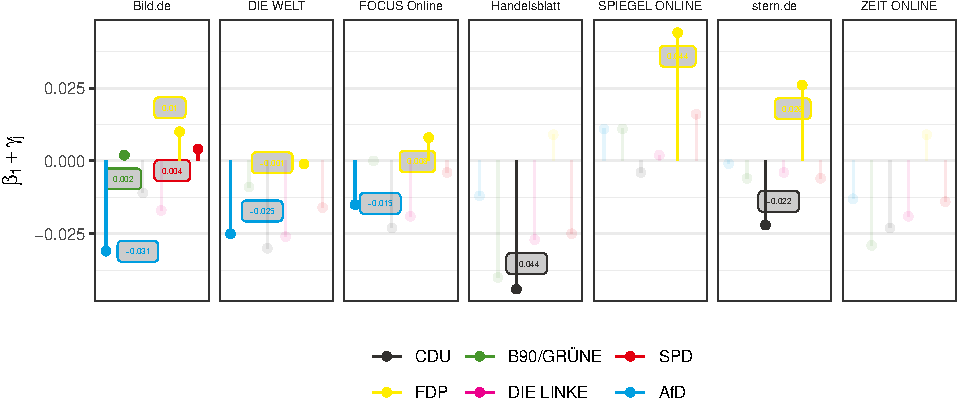
\includegraphics[width=1\linewidth]{main_text_files/figure-latex/Plot coefficients - RDiT dummy-1} 

}

\caption{Coefficients of RDiT dummy regression \label{fig:coeff_rdit_dummy}}\label{fig:Plot coefficients - RDiT dummy}
\end{figure}

\autoref{fig:coeff_rdit_dummy} displays the transformed coefficients of
the interaction terms. Note that the coefficient of the treatment effect
(without interaction) shows the treatment effect for AfD since it is the
base dummy group. While in the previous model without party dummies, the
treatment effect for Bild.de was not significant, the present model
shows a significant negative effect for the topic similarity for Bild.de
and AfD (\(-17\%\)), as well as a significant positive effect between
Bild.de and B90/GRÜNE (\(25\%\)), SPD (\(27.7\%\)) and FDP (\(24.4\%\)).
In the case of DIE WELT, the only significant effect is the one
regarding AfD: The topic similarity decreases by about \(15.4\%\)
shortly after election day, which roughly corresponds to the total
treatment effect found in the previous model. Also, the results show a
decrease in the topic similarity between CDU and the online news of
Handelsblatt (\(23.8\%\)), SPIEGEL ONLINE (\(15.2\%\)), and stern.de
(\(19.9\%\). In the case of Handelsblatt, a similar negative effect
exists for B90/GRÜNE (\(22.9\%\)). The same is true for ZEIT ONLINE,
where the topic similarity decreases for B90/GRÜNE right after the
election day by \(22\%\). No effect of the election day can be detected
in the case of FOCUS ONLINE on neither of the model specifications.

\hypertarget{vi-discussion-and-conclusion}{%
\section{VI Discussion and
conclusion}\label{vi-discussion-and-conclusion}}

In the run-up to the 2017 federal election, German media was accused of
indirectly influencing the election through its political coverage. On
the one hand, it was accused of providing a stage for the AfD through
its choice of topics, which led to a rise in the party's popularity.
But, on the other hand, the AfD accused the same media of devaluing the
party through negative reporting.

This paper investigates whether political reporting of German online
newspapers was similar for the major political parties during the
election campaign for the Bundestag 2017. Results show that the news
articles of all newspapers (except for Handelsblatt) are significantly
more similar to press releases of the AfD than any other party.

Although no statement can be made about the tonality with which
AfD-related issues are discussed, it can be assumed that the mere
disproportionate mention of these topics in the media has brought the
party more into the focus of voters. The assumption that the RDiT
results can partially confirm coverage changes as Election Day
approaches: Although the topic probability decreases for almost all news
providers, except for FOCUS ONLINE, there are considerable differences
with regard to the parties.

\newpage

\hypertarget{annex}{%
\section{Annex}\label{annex}}

\begin{longtable}[]{@{}lll@{}}
\caption{Online sources for press releases
\label{table:press_releases_sources}}\tabularnewline
\toprule
& Party & Parliamentary Group \\
\midrule
\endfirsthead
\toprule
& Party & Parliamentary Group \\
\midrule
\endhead
CDU & cdu.de & presseportal.de \\
SPD & spd.de & spdfraktion.de \\
FDP & fdp.de & fdpbt.de \\
B90/Die Grünen & gruene.de & gruene-bundestag.de \\
DIE LINKE & die-linke.de &
die-linke.de/start/presse/aus-dem-bundestag \\
AfD & afd.de & afdbundestag.de \\
\bottomrule
\end{longtable}

\begin{table}[!htbp] \centering 
  \caption{7 most probable terms per topic} 
  \label{table:top_terms} 
\begin{tabular}{@{\extracolsep{5pt}} cc} 
\\[-1.8ex]\hline 
\hline \\[-1.8ex] 
 & Top Terms \\ 
\hline \\[-1.8ex] 
1 & a, the, s, of, u, brexit, großbritannien \\ 
2 & merkel, angela, kanzlerin, bundeskanzlerin, cdu, merkels, deutschland \\ 
3 & spd, union, cdu, csu, koalitionsvertrag, koalitionsverhandlungen, schulz \\ 
4 & afd, weidel, gauland, alice, alexander, politiker, äußerungen \\ 
5 & stimmen, wahlkreis, kandidaten, afd, wahl, gewählt, fdp \\ 
6 & trump, us, usa, deutschland, präsident, donald, berlin \\ 
7 & cdu, union, peter, politiker, spahn, altmaier, schäuble \\ 
8 & spd, koalition, union, groko, große, koalitionsverhandlungen, parteitag \\ 
9 & afd, partei, sachsen, gauland, parteien, pazderski, höcke \\ 
10 & diesel, unternehmen, deutschland, autos, deutschen, industrie, fahrverbote \\ 
11 & ge, ten, be, le, ver, lambsdorff, te \\ 
12 & gericht, prozess, urteil, richter, staatsanwaltschaft, verfahren, jahre \\ 
13 & berlin, deutschen, osten, o, tag, jahr, millionen \\ 
14 & august, cdu, spd, prozent, bundestagswahl, wahl, parteien \\ 
15 & kohl, helmut, kohls, einheit, kanzler, tod, deutschen \\ 
16 & spd, nahles, andrea, partei, scholz, schulz, schwesig \\ 
17 & csu, seehofer, horst, söder, obergrenze, bayern, chef \\ 
18 & prozent, umfrage, spd, union, fdp, cdu, afd \\ 
19 & polizei, stadt, menschen, polizisten, täter, verletzt, angaben \\ 
20 & euro, milliarden, jahr, millionen, prozent, bund, geld \\ 
21 & grünen, linke, linken, özdemir, partei, wagenknecht, göring \\ 
22 & cdu, niedersachsen, spd, grünen, rot, fdp, landtag \\ 
23 & welt, politik, menschen, jahren, lange, frage, fragen \\ 
24 & g, hamburg, gipfel, polizei, hamburger, demonstranten, scholz \\ 
25 & deutschland, is, verfassungsschutz, syrien, gefährder, islamisten, staat \\ 
26 & steinmeier, schmidt, russland, frank, bundespräsident, glyphosat, walter \\ 
27 & afd, petry, partei, fraktion, frauke, meuthen, gauland \\ 
28 & berliner, berlin, amri, maizière, innenminister, behörden, daten \\ 
29 & gabriel, sigmar, außenminister, spd, schröder, amt, gerhard \\ 
30 & bundestag, spd, abgeordneten, abgeordnete, parlament, abstimmung, fraktion \\ 
31 & türkei, erdogan, türkischen, deutschland, bundesregierung, türkische, deutsche \\ 
32 & frauen, deutschland, kinder, studie, eltern, muslime, antisemitismus \\ 
33 & fdp, jamaika, lindner, koalition, neuwahlen, spd, grünen \\ 
34 & facebook, maas, twitter, gesetz, internet, netz, heiko \\ 
35 & eu, deutschland, europa, bundesregierung, europäischen, deutschen, menschen \\ 
36 & bundeswehr, soldaten, leyen, nato, ursula, einsatz, verteidigungsministerin \\ 
37 & schulz, spd, martin, kanzlerkandidat, wahlkampf, bundestagswahl, partei \\ 
38 & flüchtlinge, deutschland, menschen, zahl, flüchtlingen, familiennachzug, jahr \\ 
39 & fdp, grünen, jamaika, csu, union, grüne, cdu \\ 
40 & bundestagswahl, afd, wahl, prozent, partei, bundestag, parteien \\ 
\hline \\[-1.8ex] 
\end{tabular} 
\end{table}

\begin{figure}

{\centering 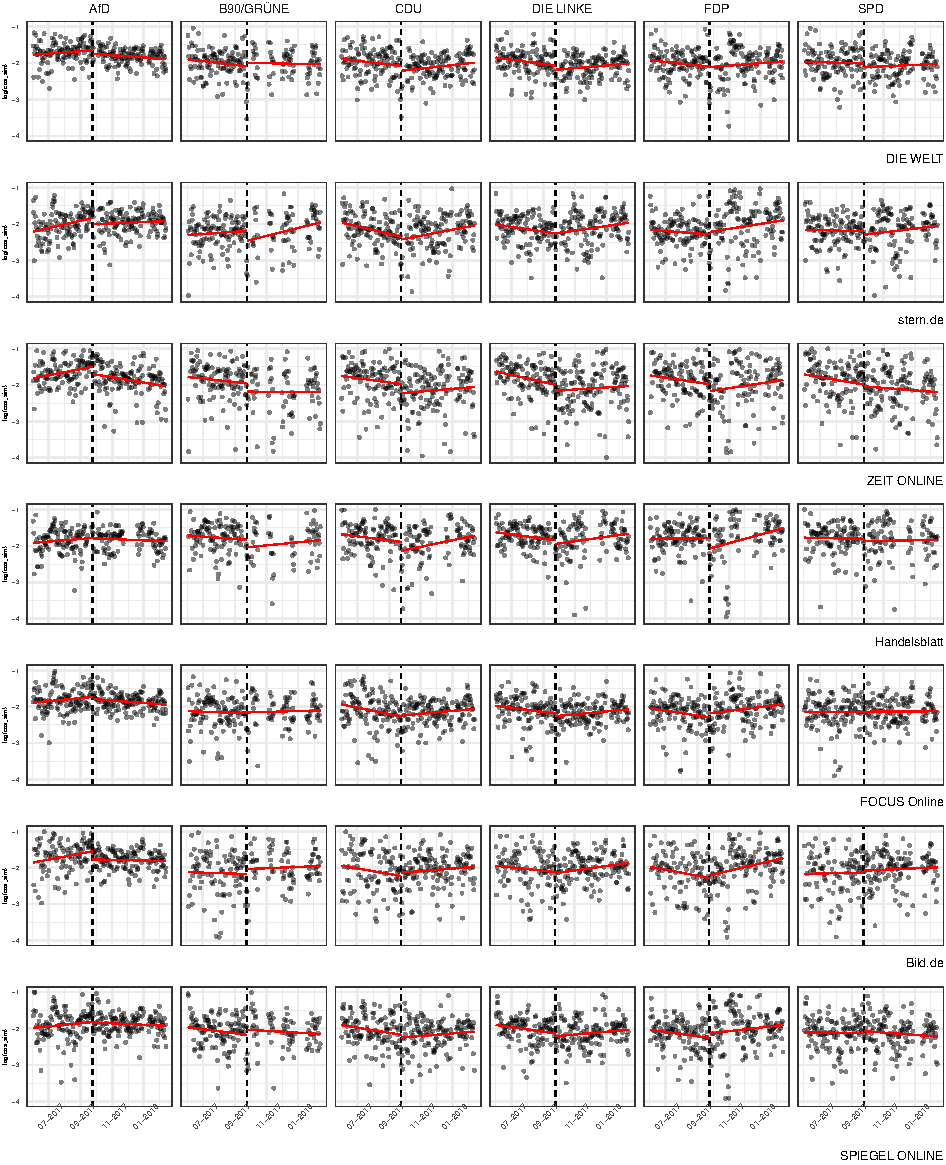
\includegraphics[width=1\linewidth]{main_text_files/figure-latex/Daily mean cosine similarity - cutoff value-1} 

}

\caption{Log of daily mean cosine similarity between newspaper/press articles pairs - with cutoff value \label{fig:mean_cosine_sim_rd}}\label{fig:Daily mean cosine similarity - cutoff value}
\end{figure}

\newpage

\hypertarget{references}{%
\section*{References}\label{references}}
\addcontentsline{toc}{section}{References}

\hypertarget{refs}{}
\begin{CSLReferences}{1}{0}
\leavevmode\hypertarget{ref-angrist_using_1999}{}%
Angrist, Joshua D., and Victor Lavy. 1999. {``Using Maimonides' Rule to
Estimate the Effect of Class Size on Scholastic Achievement.''}
\emph{The Quarterly Journal of Economics} 114 (2): 533--75.
\url{https://www.jstor.org/stable/2587016}.

\leavevmode\hypertarget{ref-bholat_text_2015}{}%
Bholat, David M., Stephen Hansen, Pedro M. Santos, and Cheryl
Schonhardt-Bailey. 2015. {``Text Mining for Central Banks.''}
\emph{{SSRN} Electronic Journal}, June.
\url{http://www.academia.edu/13430482/Text_mining_for_central_banks}.

\leavevmode\hypertarget{ref-blassnig_hitting_2019}{}%
Blassnig, Sina, Sven Engesser, Nicole Ernst, and Frank Esser. 2019.
{``Hitting a Nerve: Populist News Articles Lead to More Frequent and
More Populist Reader Comments.''} \emph{Political Communication},
August, 1--23. \url{https://doi.org/10.1080/10584609.2019.1637980}.

\leavevmode\hypertarget{ref-blei_latent_2003}{}%
Blei, David M., Andrew Y Ng, and Michael I Jordan. 2003. {``Latent
Dirichlet Allocation.''} \emph{Journal of Machine Learning Research} 3
(January): 993--1022.

\leavevmode\hypertarget{ref-braun_variational_2010}{}%
Braun, Michael, and Jon McAuliffe. 2010. {``Variational Inference for
Large-Scale Models of Discrete Choice.''} \emph{Journal of the American
Statistical Association} 105 (489): 324--35.
\url{https://doi.org/10.1198/jasa.2009.tm08030}.

\leavevmode\hypertarget{ref-dewenter_einfuhrung_2014}{}%
Dewenter, Ralf, and Jürgen Rösch. 2014. \emph{Einführung in die neue
Ökonomie der Medienmärkte: Eine wettbewerbsökonomische Betrachtung aus
Sicht der Theorie der zweiseitigen Märkte}. Springer-Verlag.

\leavevmode\hypertarget{ref-druckman_impact_2005}{}%
Druckman, James N., and Michael Parkin. 2005. {``The Impact of Media
Bias: How Editorial Slant Affects Voters.''} \emph{The Journal of
Politics} 67 (4): 1030--49.
\url{https://doi.org/10.1111/j.1468-2508.2005.00349.x}.

\leavevmode\hypertarget{ref-eberl_lying_2018}{}%
Eberl, Jakob-Moritz. 2018. {``Lying Press: Three Levels of Perceived
Media Bias and Their Relationship with Political Preferences.''}
\emph{Communications}, March.
\url{https://doi.org/10.1515/commun-2018-0002}.

\leavevmode\hypertarget{ref-eberl_one_2017}{}%
Eberl, Jakob-Moritz, Hajo G. Boomgaarden, and Markus Wagner. 2017.
{``One Bias Fits All? Three Types of Media Bias and Their Effects on
Party Preferences.''} \emph{Communication Research} 44 (8): 1125--48.
\url{https://doi.org/10.1177/0093650215614364}.

\leavevmode\hypertarget{ref-erosheva_mixed-membership_2004}{}%
Erosheva, Elena, Stephen Fienberg, and John Lafferty. 2004.
{``Mixed-Membership Models of Scientific Publications.''}
\emph{Proceedings of the National Academy of Sciences} 101 (June):
5220--27. \url{https://doi.org/10.1073/pnas.0307760101}.

\leavevmode\hypertarget{ref-gentzkow_media_2004}{}%
Gentzkow, Matthew A., and Jesse M. Shapiro. 2004. {``Media, Education
and Anti-Americanism in the Muslim World.''} \emph{Journal of Economic
Perspectives} 18 (3): 117--33.
\url{https://doi.org/10.1257/0895330042162313}.

\leavevmode\hypertarget{ref-gentzkow_text_2017}{}%
Gentzkow, Matthew, Bryan T. Kelly, and Matt Taddy. 2017. {``Text as
Data.''} Working Paper 23276. National Bureau of Economic Research.
\url{https://doi.org/10.3386/w23276}.

\leavevmode\hypertarget{ref-griffiths_probabilistic_2002}{}%
Griffiths, Thomas L., and Mark Steyvers. 2002. {``A Probabilistic
Approach to Semantic Representation.''} \emph{Proceedings of the Annual
Meeting of the Cognitive Science Society} 24 (24).
\url{https://escholarship.org/uc/item/44x9v7m7}.

\leavevmode\hypertarget{ref-griffiths_finding_2004}{}%
---------. 2004. {``Finding Scientific Topics.''} \emph{Proceedings of
the National Academy of Sciences} 101 (June): 5228--35.
\url{https://doi.org/10.1073/pnas.0307752101}.

\leavevmode\hypertarget{ref-grimmer_text_2013}{}%
Grimmer, Justin, and Brandon Stewart. 2013. {``Text as Data: The Promise
and Pitfalls of Automatic Content Analysis Methods for Political
Texts.''} \emph{Political Analysis} 21: 267--97.

\leavevmode\hypertarget{ref-groseclose_measure_2005}{}%
Groseclose, Tim, and Jeffrey Milyo. 2005. {``A Measure of Media Bias.''}
\emph{The Quarterly Journal of Economics} 120 (4): 1191--1237.
\url{https://www.jstor.org/stable/25098770}.

\leavevmode\hypertarget{ref-hahn_identification_2001}{}%
Hahn, Jinyong, Petra Todd, and Wilbert Van der Klaauw. 2001.
{``Identification and Estimation of Treatment Effects with a
Regression-Discontinuity Design.''} \emph{Econometrica} 69 (1): 201--9.
\url{https://www.jstor.org/stable/2692190}.

\leavevmode\hypertarget{ref-hlavac_stargazer_2018}{}%
Hlavac, Marek. 2018. \emph{Stargazer: Well-Formatted Regression and
Summary Statistics Tables. R Package Version 5.2.2}.
\url{https://CRAN.R-project.org/package=stargazer}.

\leavevmode\hypertarget{ref-hofmann_probabilistic_1999}{}%
Hofmann, Thomas. 1999. {``Probabilistic Latent Semantic Indexing.''} In
\emph{Proceedings of the 22Nd Annual International {ACM} {SIGIR}
Conference on Research and Development in Information Retrieval},
50--57. {SIGIR} '99. New York, {NY}, {USA}: {ACM}.
\url{https://doi.org/10.1145/312624.312649}.

\leavevmode\hypertarget{ref-imbens_regression_2008}{}%
Imbens, Guido W., and Thomas Lemieux. 2008. {``Regression Discontinuity
Designs: A Guide to Practice.''} \emph{Journal of Econometrics}, The
regression discontinuity design: Theory and applications, 142 (2):
615--35. \url{https://doi.org/10.1016/j.jeconom.2007.05.001}.

\leavevmode\hypertarget{ref-jacob_practical_2012}{}%
Jacob, Robin, Pei Zhu, Marie-Andrée Somers, and Howard Bloom. 2012.
\emph{A Practical Guide to Regression Discontinuity}. {MDRC}.
\url{https://eric.ed.gov/?id=ED565862}.

\leavevmode\hypertarget{ref-kepplinger_einfluss_2004}{}%
Kepplinger, Hans Mathias, and Marcus Maurer. 2004. {``Der Einfluss Der
Pressemitteilungen Der Bundesparteien Auf Die Berichterstattung Im
Bundestagswahlkampf 2002.''} In \emph{Quo Vadis Public Relations? Auf
Dem Weg Zum Kommunikationsmanagement: Bestandsaufnahmen Und
Entwicklungen}, edited by Juliana Raupp and Joachim Klewes, 113--24.
Wiesbaden: {VS} Verlag für Sozialwissenschaften.
\url{https://doi.org/10.1007/978-3-322-83381-5_9}.

\leavevmode\hypertarget{ref-van_der_klaauw_estimating_2002}{}%
Klaauw, Wilbert van der. 2002. {``Estimating the Effect of Financial Aid
Offers on College Enrollment: A Regression-Discontinuity Approach.''}
\emph{International Economic Review} 43 (4): 1249--87.
\url{https://www.jstor.org/stable/826967}.

\leavevmode\hypertarget{ref-lee_regression_2010}{}%
Lee, David S., and Thomas Lemieux. 2010. {``Regression Discontinuity
Designs in Economics.''} \emph{Journal of Economic Literature} 48 (2):
281--355. \url{https://doi.org/10.1257/jel.48.2.281}.

\leavevmode\hypertarget{ref-lengauer_candidate_2013}{}%
Lengauer, Günther, and David Johann. 2013. {``Candidate and Party Bias
in the News and Its Effects on Party Choice: Evidence from Austria.''}
\emph{Studies in Communication Sciences} 13 (1): 41--49.
\url{https://doi.org/10.1016/j.scoms.2013.04.011}.

\leavevmode\hypertarget{ref-lott_is_2014}{}%
Lott, John R., and Kevin A. Hassett. 2014. {``Is Newspaper Coverage of
Economic Events Politically Biased?''} \emph{Public Choice} 160 (1):
65--108. \url{https://doi.org/10.1007/s11127-014-0171-5}.

\leavevmode\hypertarget{ref-mimno_optimizing_2011}{}%
Mimno, David, Hanna M. Wallach, Edmund Talley, Miriam Leenders, and
Andrew McCallum. 2011. {``Optimizing Semantic Coherence in Topic
Models.''} In \emph{Proceedings of the Conference on Empirical Methods
in Natural Language Processing}, 262--72. {EMNLP} '11. Stroudsburg,
{PA}, {USA}: Association for Computational Linguistics.
\url{http://dl.acm.org/citation.cfm?id=2145432.2145462}.

\leavevmode\hypertarget{ref-newman_automatic_2010}{}%
Newman, David, Jey Han Lau, Karl Grieser, and Timothy Baldwin. 2010.
{``Automatic Evaluation of Topic Coherence.''} In \emph{Human Language
Technologies: The 2010 Annual Conference of the North American Chapter
of the Association for Computational Linguistics}, 100--108. {HLT} '10.
Stroudsburg, {PA}, {USA}: Association for Computational Linguistics.
\url{http://dl.acm.org/citation.cfm?id=1857999.1858011}.

\leavevmode\hypertarget{ref-newman_reuters_2018}{}%
Newman, Nic, Richard Fletcher, Antonis Kalogeropoulos, David Levy, and
Rasmus Kleis Nielsen. 2018. {``Reuters Institute Digital News Report
2018.''} Reuters Institute for the Study of Journalism.
\url{http://media.digitalnewsreport.org/wp-content/uploads/2018/06/digital-news-report-2018.pdf?x89475}.

\leavevmode\hypertarget{ref-ramage_characterizing_2010}{}%
Ramage, Daniel, Susan Dumais, and Daniel Liebling. 2010.
\emph{Characterizing Microblogs with Topic Models}.

\leavevmode\hypertarget{ref-rehs_structural_2020}{}%
Rehs, Andreas. 2020. {``A Structural Topic Model Approach to Scientific
Reorientation of Economics and Chemistry After German Reunification.''}
\emph{Scientometrics} 125 (2): 1229--51.
\url{https://doi.org/10.1007/s11192-020-03640-0}.

\leavevmode\hypertarget{ref-roberts_model_2016}{}%
Roberts, Margaret E., Brandon M. Stewart, and Edoardo M. Airoldi. 2016.
{``A Model of Text for Experimentation in the Social Sciences.''}
\emph{Journal of the American Statistical Association} 111 (515):
988--1003. \url{https://doi.org/10.1080/01621459.2016.1141684}.

\leavevmode\hypertarget{ref-roberts_navigating_2016}{}%
Roberts, Margaret, Brandon Stewart, and Dustin Tingley. 2016a.
{``Navigating the Local Modes of Big Data: The Case of Topic Models.''}
In \emph{Computational Social Science: Discovery and Prediction}. New
York: Cambridge University Press.

\leavevmode\hypertarget{ref-roberts_stm:_2016}{}%
---------. 2016b. {``Stm: R Package for Structural Topic Models.''}
\emph{Journal of Statistical Software} forthcoming (January).

\leavevmode\hypertarget{ref-stromback_four_2008}{}%
Strömbäck, Jesper. 2008. {``Four Phases of Mediatization: An Analysis of
the Mediatization of Politics.''} \emph{The International Journal of
Press/Politics} 13 (3): 228--46.
\url{https://doi.org/10.1177/1940161208319097}.

\leavevmode\hypertarget{ref-taddy_estimation_2012}{}%
Taddy, Matt. 2012. {``On Estimation and Selection for Topic Models.''}
In \emph{Proceedings of the 15th International Conference on Artificial
Intelligence and Statistics}.

\leavevmode\hypertarget{ref-takens_media_2013}{}%
Takens, Janet, Wouter Atteveldt, Anita van Hoof, and Jan Kleinnijenhuis.
2013. {``Media Logic in Election Campaign Coverage.''} \emph{European
Journal of Communication} 28 (June): 277--93.
\url{https://doi.org/10.1177/0267323113478522}.

\leavevmode\hypertarget{ref-thistlethwaite_regression-discontinuity_1960}{}%
Thistlethwaite, Donald L., and Donald T. Campbell. 1960.
{``Regression-Discontinuity Analysis: An Alternative to the Ex Post
Facto Experiment.''} \emph{Journal of Educational Psychology} 51 (6):
309--17. \url{https://doi.org/10.1037/h0044319}.

\leavevmode\hypertarget{ref-wallach_rethinking_2009}{}%
Wallach, Hanna M., David M. Mimno, and Andrew McCallum. 2009.
{``Rethinking {LDA}: Why Priors Matter.''} In \emph{Advances in Neural
Information Processing Systems 22}, edited by Y. Bengio, D. Schuurmans,
J. D. Lafferty, C. K. I. Williams, and A. Culotta, 1973--81. Curran
Associates, Inc.
\url{http://papers.nips.cc/paper/3854-rethinking-lda-why-priors-matter.pdf}.

\end{CSLReferences}

\end{document}
